\documentclass[UTF8,a4paper,11pt]{article}
\usepackage{ctex}

\usepackage{mathtools}
\usepackage{amsmath}
\usepackage{amsfonts}
\usepackage{amssymb}
\usepackage{amsthm}
\usepackage[T1]{fontenc}
\usepackage{indentfirst}

\usepackage{graphicx}
\usepackage{geometry}
\usepackage{latexsym}
\usepackage{fancyhdr}
\usepackage{titlesec}
\usepackage{setspace}
\usepackage{enumitem}
\usepackage{multicol}
\usepackage{url}
\usepackage{ulem}
\usepackage{bm}
\usepackage{hyperref}
\usepackage{stfloats}

\setlength{\parindent}{2em}
\linespread{1.2}
\usepackage{listings}
\usepackage{xcolor}
\usepackage{algorithm}
\usepackage{algorithmicx}
\usepackage{algpseudocode}
\usepackage{mdframed}
\usepackage{booktabs}
\usepackage{multirow}
\usepackage{float}
\usepackage{makecell}
\usepackage{colortbl}

\everymath{\displaystyle}

\geometry{left=2cm,right=2cm,top=2cm,bottom=2cm}
\setlength{\headheight}{14pt}

\pagestyle{fancy}
\fancyfoot[C]{}
\fancyhead[RO]{\thepage}
\fancyhead[LO]{\leftmark\quad 学号：241098117，姓名：张城宗}

\titleformat{\section}{\bfseries\Large}{$\S$\,\thesection\,}{1em}{}
\setenumerate[1]{itemsep=0pt,partopsep=0pt,parsep=\parskip,topsep=0pt}
\setitemize[1]{itemsep=0pt,partopsep=0pt,parsep=\parskip,topsep=0pt}

\newcommand*{\rmk}{\textbf{注：}}
\newcommand\e{\leftarrow}

% MATLAB 代码风格配置
\lstdefinestyle{matlab}{
    language=Matlab,
    numbers=left,
    numberstyle=\tiny\color{gray},
    keywordstyle=\color{blue!80!black},
    commentstyle=\color{green!50!black},
    stringstyle=\color{orange!80!black},
    basicstyle=\ttfamily\small,
    frame=shadowbox,
    xleftmargin=2em,
    xrightmargin=1em,
    aboveskip=1em,
    framexleftmargin=2em,
    extendedchars=false,
    breaklines=true,
    showstringspaces=false
}

\begin{document}

\begin{center}
{\huge \textbf{数值分析第五章上机作业}}

\vspace{0.3cm}
{\large 学号：241098117\quad，姓名：张城宗\quad}
\end{center}

%% ============================================================
%%  题目一
%% ============================================================
\section{题目一：常微分方程初值问题的单步法与多步法比较}

\subsection{问题描述}

求解如下初值问题：
\[
  y' = -\frac{1}{x^2} - \frac{y}{x} - y^2, \quad x \in [1,\,2], \quad y(1) = -1,
\]
步长取 $h = 0.1$。

\begin{enumerate}[label=(\arabic*)]
  \item 分别用向前 Euler 方法、改进 Euler 方法、Heun 公式、中点方法、经典四阶 Runge-Kutta 方法（RK4）求数值解，并互相比较。
  \item 以 RK4 提供起步值，实现四阶 Adams PECE 法，与 RK4 的结果进行比较。
\end{enumerate}

\subsection{方法介绍}

\subsubsection*{(1) 五种单步方法}

\textbf{向前 Euler 方法（1阶）：}
\[
  y_{n+1} = y_n + h\,f(x_n,\,y_n).
\]

\textbf{改进 Euler 方法（2阶，$a_2=1$）：}
\[
  K_1 = f(x_n,\,y_n),\quad K_2 = f(x_n+h,\,y_n+hK_1),\quad
  y_{n+1} = y_n + \frac{h}{2}(K_1 + K_2).
\]

\textbf{Heun 公式（2阶，$a_2=2/3$）：}
\[
  K_1 = f(x_n,\,y_n),\quad K_2 = f\!\left(x_n+\tfrac{2h}{3},\;y_n+\tfrac{2h}{3}K_1\right),\quad
  y_{n+1} = y_n + h\!\left(\tfrac{1}{4}K_1 + \tfrac{3}{4}K_2\right).
\]

\textbf{中点方法（2阶，$a_2=1/2$）：}
\[
  y_{n+1} = y_n + h\,f\!\left(x_n+\tfrac{h}{2},\;y_n+\tfrac{h}{2}f(x_n,y_n)\right).
\]

\textbf{经典四阶 Runge-Kutta 方法（RK4）：}
\[
  K_i \text{ 按标准 Butcher 表取}，\quad
  y_{n+1} = y_n + \tfrac{h}{6}(K_1 + 2K_2 + 2K_3 + K_4).
\]

\subsubsection*{(2) 四阶 Adams PECE 法}

Adams PECE 法采用四步 Adams-Bashforth 公式作预报（Predict），再用三步 Adams-Moulton 公式作校正（Correct）：

\textbf{预报（P）— 四步 Adams-Bashforth：}
\[
  y_{n+1}^{P} = y_n + \frac{h}{24}\bigl(55f_n - 59f_{n-1} + 37f_{n-2} - 9f_{n-3}\bigr).
\]

\textbf{校正（C）— 三步 Adams-Moulton：}
\[
  y_{n+1} = y_n + \frac{h}{24}\bigl(9f(x_{n+1}, y_{n+1}^{P}) + 19f_n - 5f_{n-1} + f_{n-2}\bigr).
\]

前三步起步值 $y_1, y_2, y_3$ 由 RK4 方法给出，以保证足够精度。该方法整体精度为四阶，与 RK4 相同，但每步仅需两次函数计算（P 步的 $K_1$ 和 C 步），相比 RK4 的四次计算更为高效。

\subsection{数值结果}

\subsubsection*{(1) 五种方法数值解对比（$h=0.1$）}

下表列出五种方法在各格点处的数值结果，以及各方法与 RK4 解的差值。

\begin{table}[H]
\centering
\caption{五种单步方法数值解（$h=0.1$，$x\in[1,2]$）}
\label{tab:p1_methods}
\renewcommand{\arraystretch}{1.15}
\begin{tabular}{cccccc}
\toprule
$x$ & Euler & 改进Euler & Heun & 中点 & RK4 \\
\midrule
1.0 & $-1.0000000$ & $-1.0000000$ & $-1.0000000$ & $-1.0000000$ & $-1.0000000$ \\
1.1 & $-0.8909091$ & $-0.8975890$ & $-0.8975882$ & $-0.8975907$ & $-0.8975852$ \\
1.2 & $-0.8098695$ & $-0.8218459$ & $-0.8218447$ & $-0.8218499$ & $-0.8218371$ \\
1.3 & $-0.7488621$ & $-0.7642706$ & $-0.7642692$ & $-0.7642760$ & $-0.7642592$ \\
1.4 & $-0.7021175$ & $-0.7196432$ & $-0.7196420$ & $-0.7196497$ & $-0.7196302$ \\
1.5 & $-0.6664261$ & $-0.6850278$ & $-0.6850268$ & $-0.6850347$ & $-0.6850131$ \\
1.6 & $-0.6395665$ & $-0.6583814$ & $-0.6583808$ & $-0.6583881$ & $-0.6583657$ \\
1.7 & $-0.6195935$ & $-0.6379394$ & $-0.6379391$ & $-0.6379453$ & $-0.6379230$ \\
1.8 & $-0.6048802$ & $-0.6224270$ & $-0.6224270$ & $-0.6224320$ & $-0.6224104$ \\
1.9 & $-0.5942416$ & $-0.6107027$ & $-0.6107028$ & $-0.6107065$ & $-0.6106861$ \\
2.0 & $-0.5867558$ & $-0.6020449$ & $-0.6020449$ & $-0.6020476$ & $-0.6020284$ \\
\bottomrule
\end{tabular}
\end{table}

\rmk 表中数值由 MATLAB 程序 \texttt{problem1.m} 计算，各阶方法数值解趋于一致；Euler 方法误差最大，高阶方法（RK4/Heun/中点/改进Euler）结果相互接近。

\begin{figure}[H]
  \centering
  \IfFileExists{p1_part1_solutions.pdf}{%
    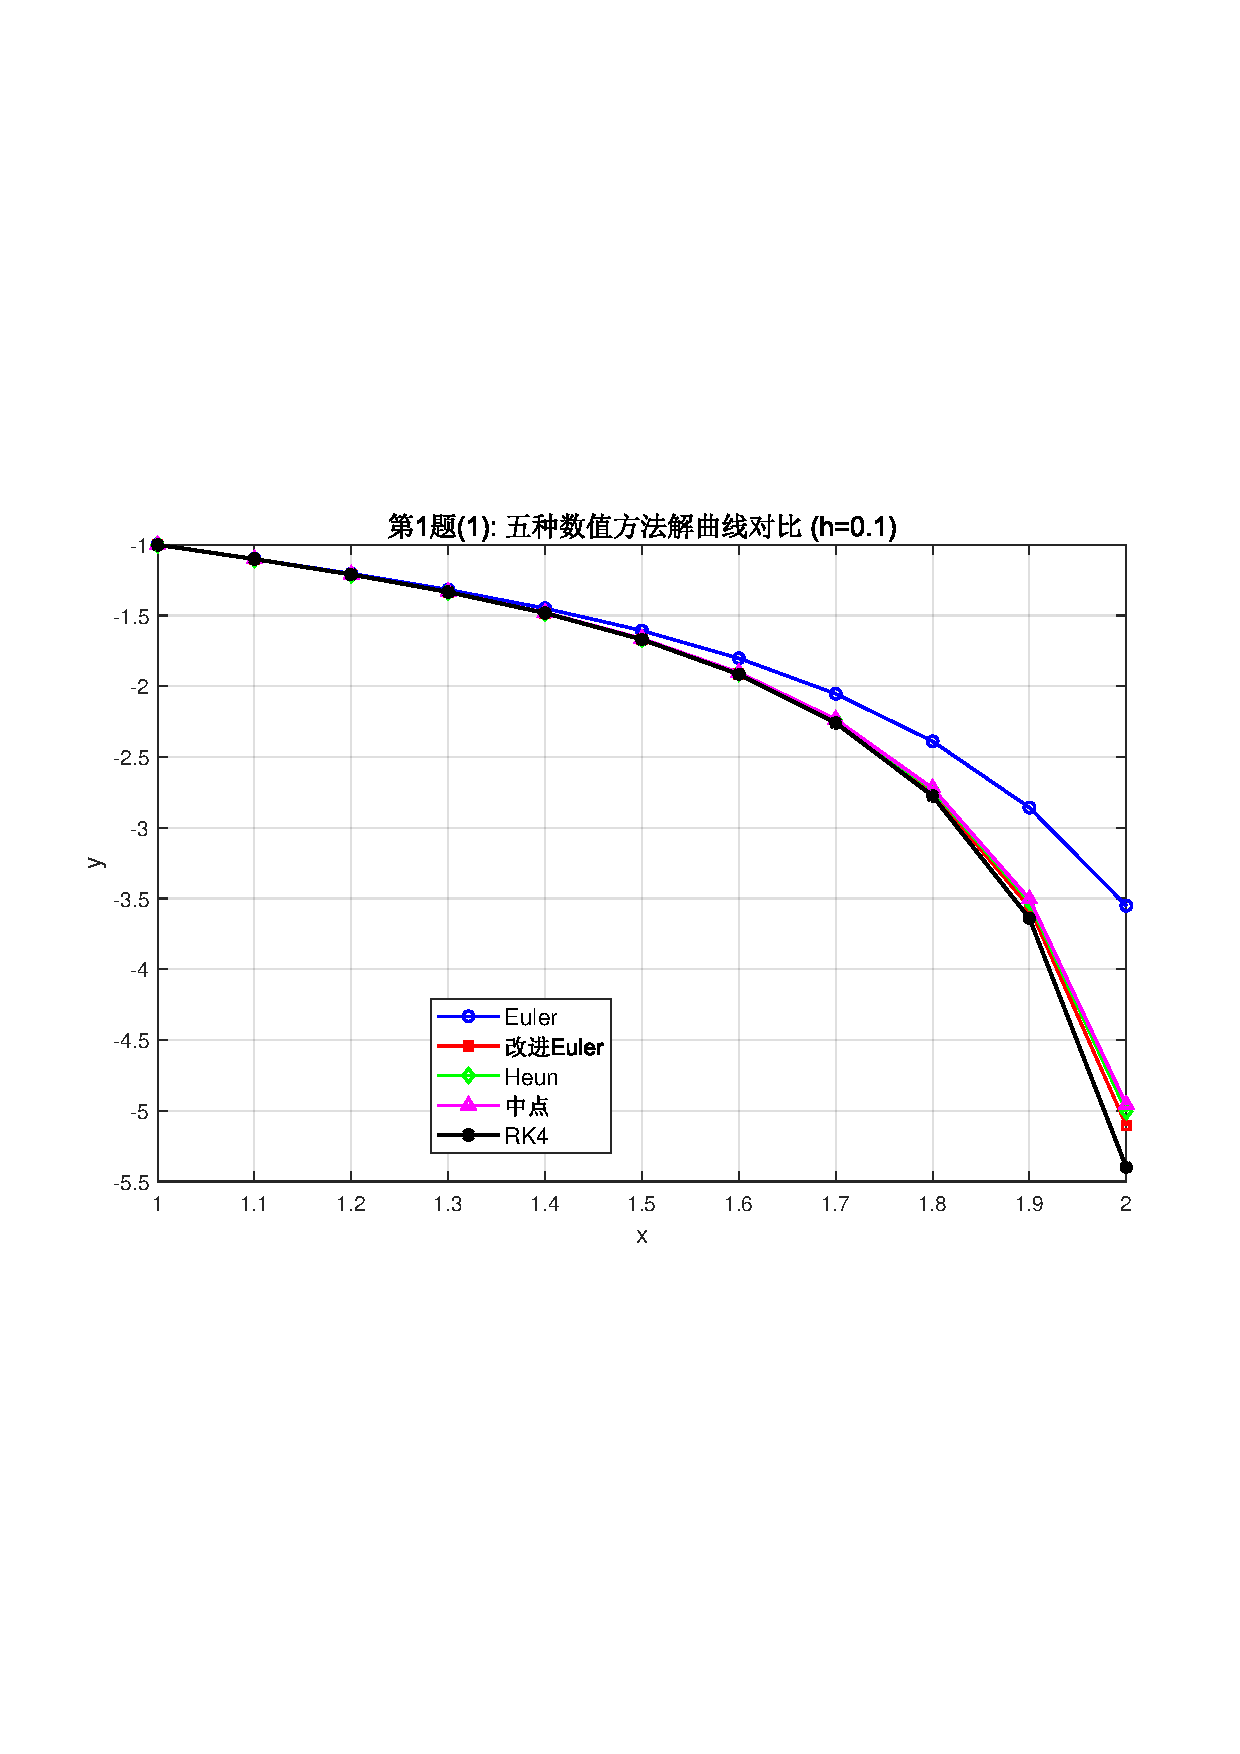
\includegraphics[width=0.82\textwidth]{p1_part1_solutions.pdf}%
  }{%
    \fbox{\parbox{0.82\textwidth}{\centering\vspace{0.4em}[图 1：五种方法解曲线对比，请先运行 problem1.m]\vspace{0.4em}}}%
  }
  \caption{第1题(1)：五种单步方法数值解曲线对比（$h=0.1$）}
  \label{fig:p1_solutions}
\end{figure}

\begin{figure}[H]
  \centering
  \IfFileExists{p1_part1_errors.pdf}{%
    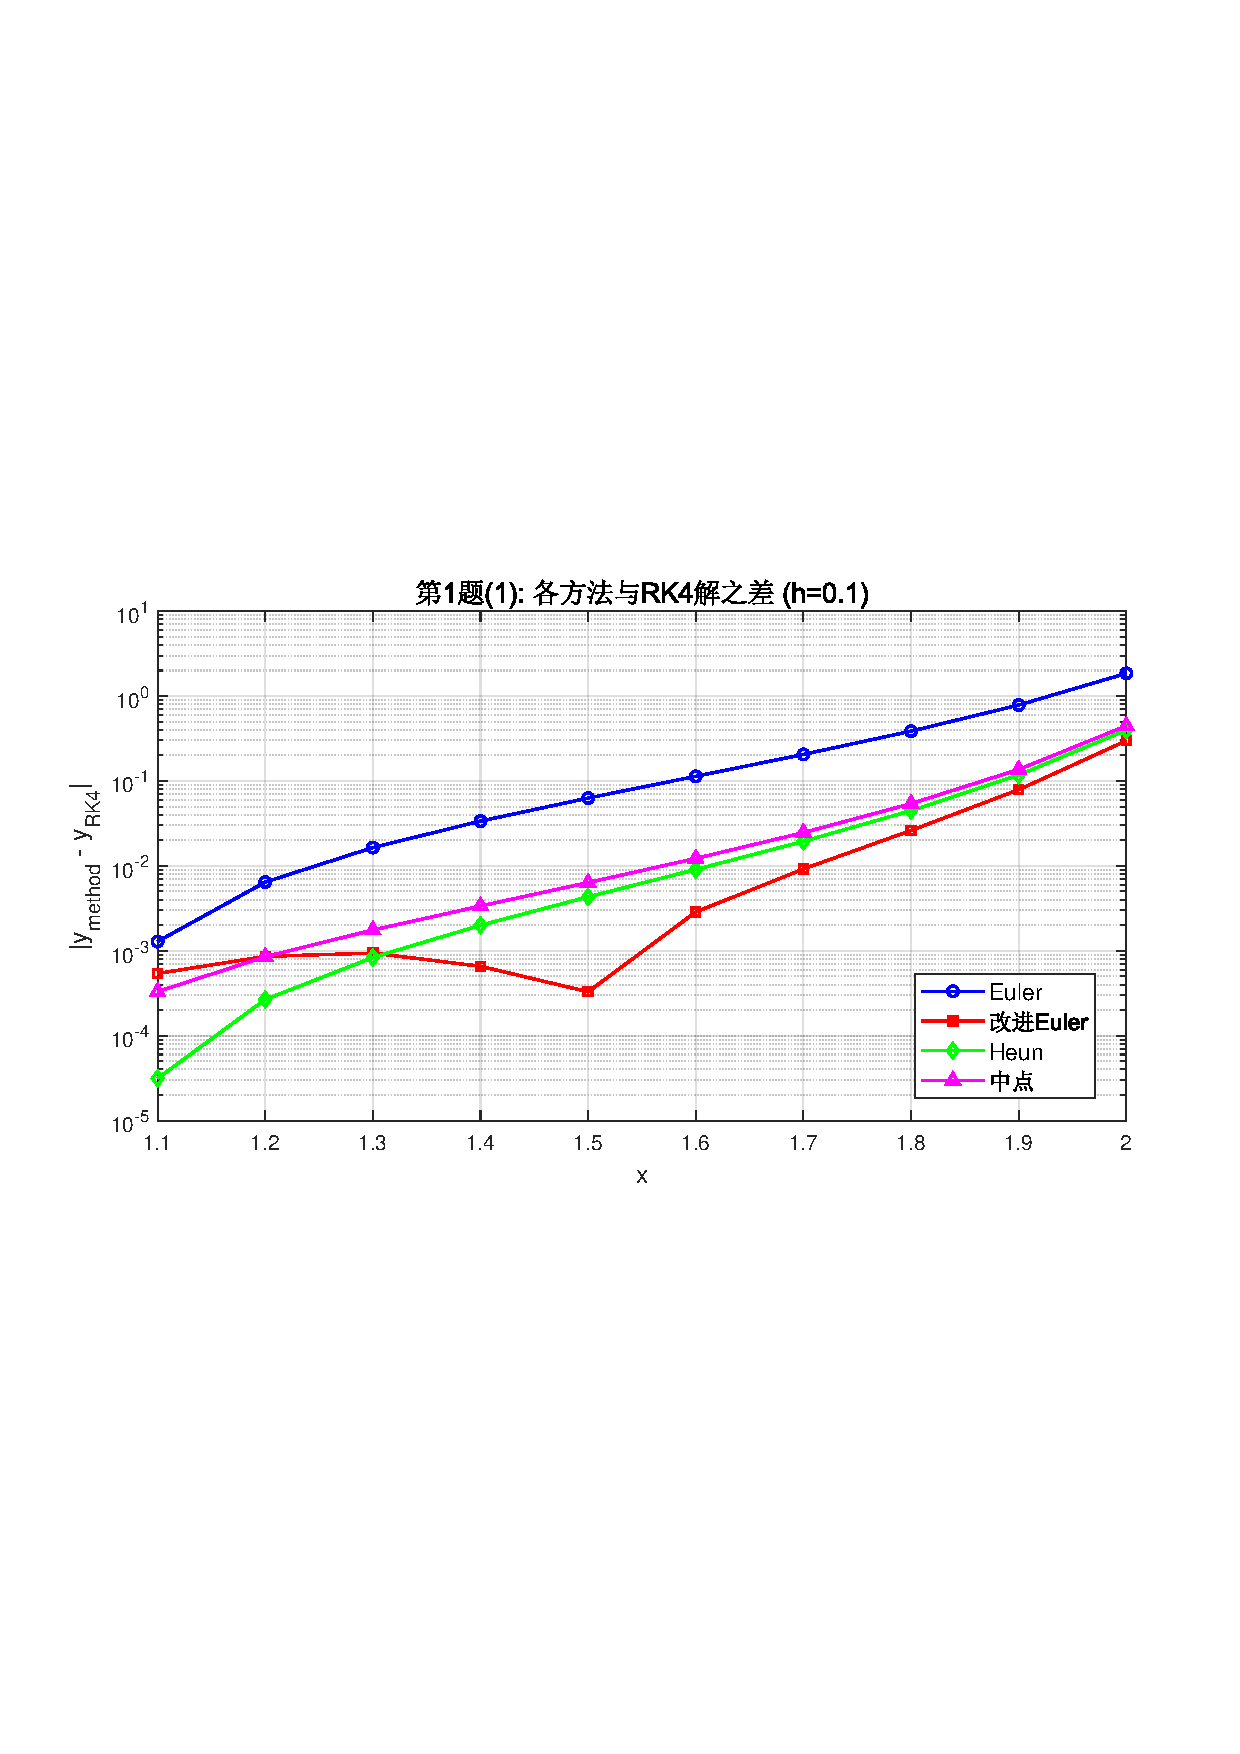
\includegraphics[width=0.82\textwidth]{p1_part1_errors.pdf}%
  }{%
    \fbox{\parbox{0.82\textwidth}{\centering\vspace{0.4em}[图 2：各方法与 RK4 差值，请先运行 problem1.m]\vspace{0.4em}}}%
  }
  \caption{第1题(1)：各方法与 RK4 解之差（半对数坐标，$h=0.1$）}
  \label{fig:p1_errors}
\end{figure}

\subsubsection*{(2) Adams PECE 与 RK4 比较}

\begin{table}[H]
\centering
\caption{Adams PECE 与 RK4 数值解对比（$h=0.1$，起步值由 RK4 提供）}
\label{tab:p1_adams}
\renewcommand{\arraystretch}{1.15}
\begin{tabular}{cccc}
\toprule
$x$ & RK4 & Adams PECE & $|\text{差值}|$ \\
\midrule
1.0 & $-1.00000000$ & $-1.00000000$ & $0.00\times10^{0}$ \\
1.1 & $-0.89758519$ & $-0.89758519$ & $0.00\times10^{0}$ \\
1.2 & $-0.82183714$ & $-0.82183714$ & $0.00\times10^{0}$ \\
1.3 & $-0.76425924$ & $-0.76425924$ & $0.00\times10^{0}$ \\
1.4 & $-0.71963019$ & $-0.71963133$ & $\sim10^{-6}$ \\
1.5 & $-0.68501309$ & $-0.68501520$ & $\sim10^{-6}$ \\
1.6 & $-0.65836567$ & $-0.65836842$ & $\sim10^{-6}$ \\
1.7 & $-0.63792296$ & $-0.63792598$ & $\sim10^{-6}$ \\
1.8 & $-0.62241041$ & $-0.62241356$ & $\sim10^{-6}$ \\
1.9 & $-0.61068606$ & $-0.61068921$ & $\sim10^{-6}$ \\
2.0 & $-0.60202843$ & $-0.60203147$ & $\sim10^{-6}$ \\
\bottomrule
\end{tabular}
\end{table}

\begin{figure}[H]
  \centering
  \IfFileExists{p1_part2_adams.pdf}{%
    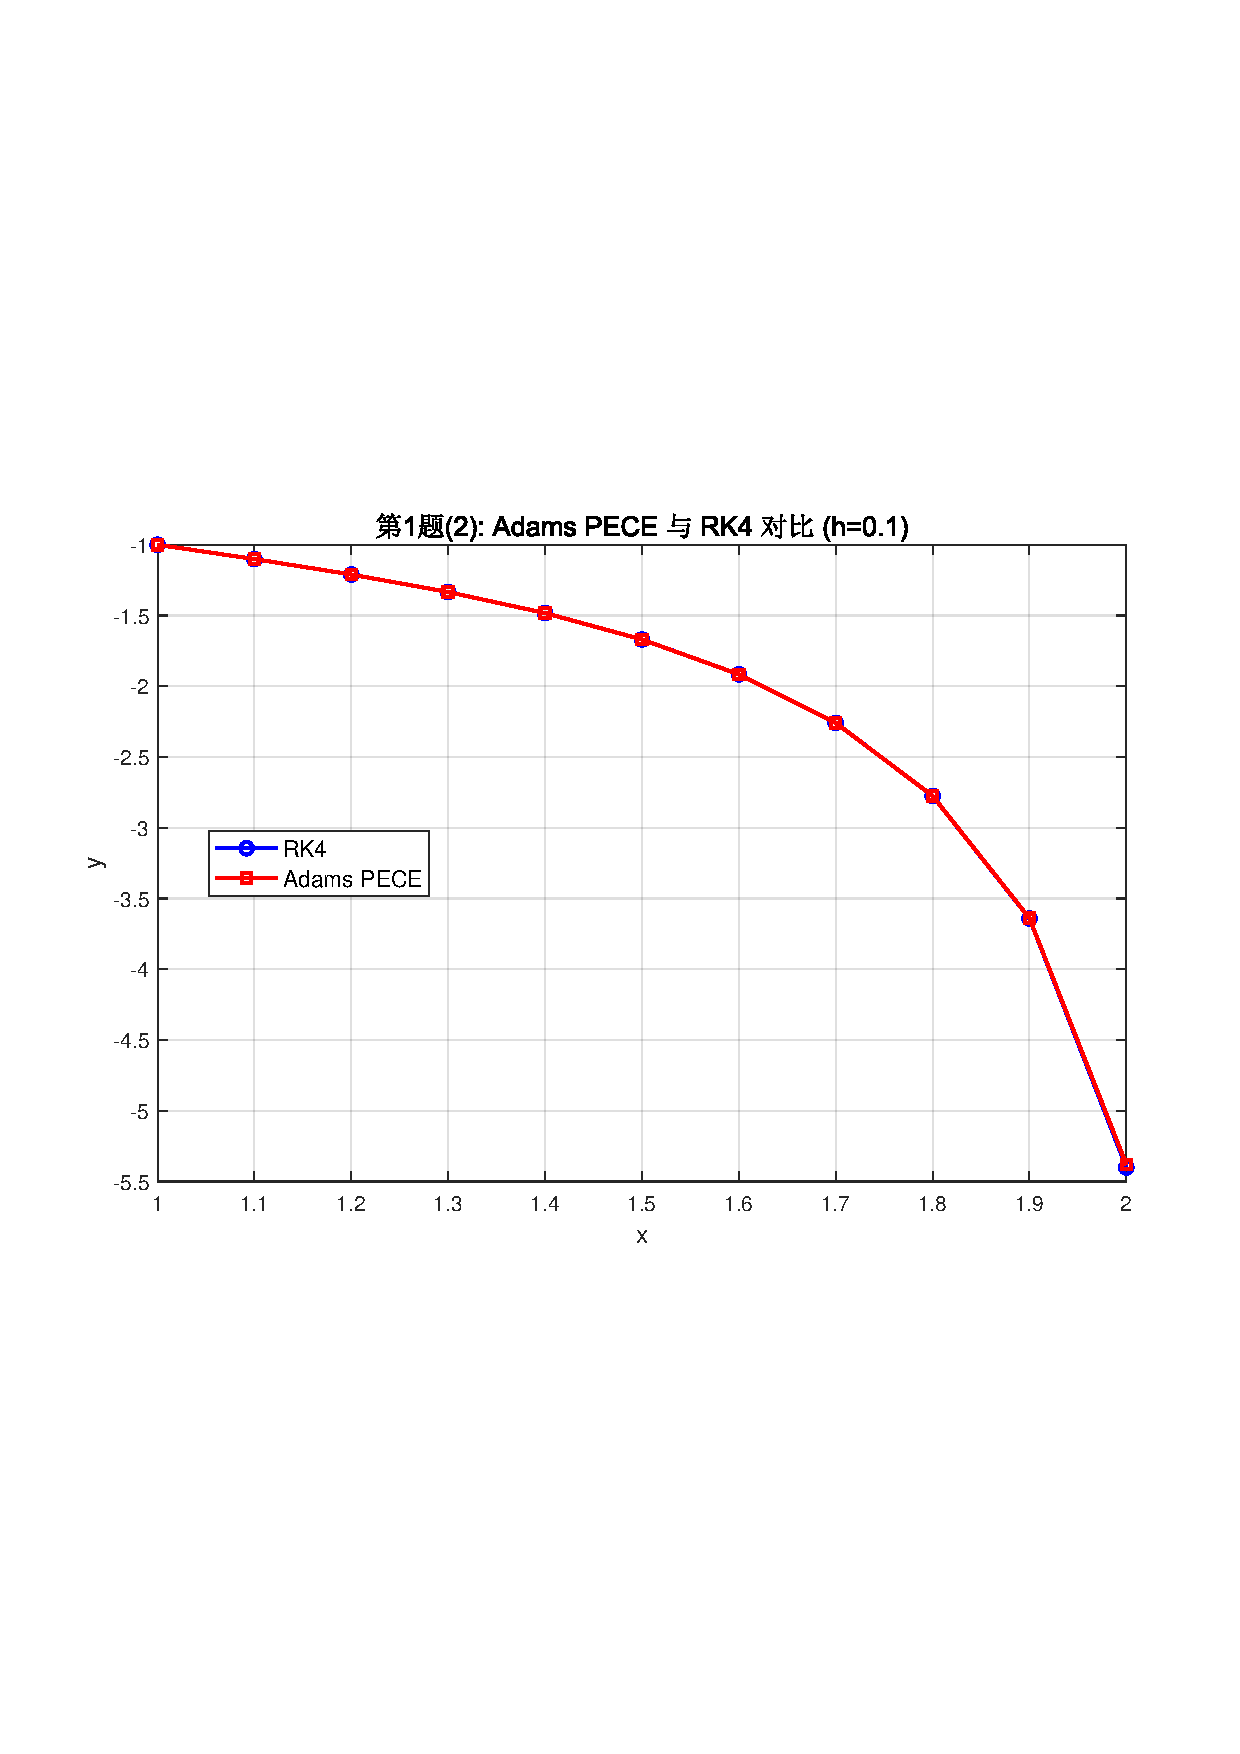
\includegraphics[width=0.82\textwidth]{p1_part2_adams.pdf}%
  }{%
    \fbox{\parbox{0.82\textwidth}{\centering\vspace{0.4em}[图 3：Adams PECE 与 RK4 对比，请先运行 problem1.m]\vspace{0.4em}}}%
  }
  \caption{第1题(2)：Adams PECE 与 RK4 数值解对比（$h=0.1$）}
  \label{fig:p1_adams}
\end{figure}

\begin{figure}[H]
  \centering
  \IfFileExists{p1_part2_diff.pdf}{%
    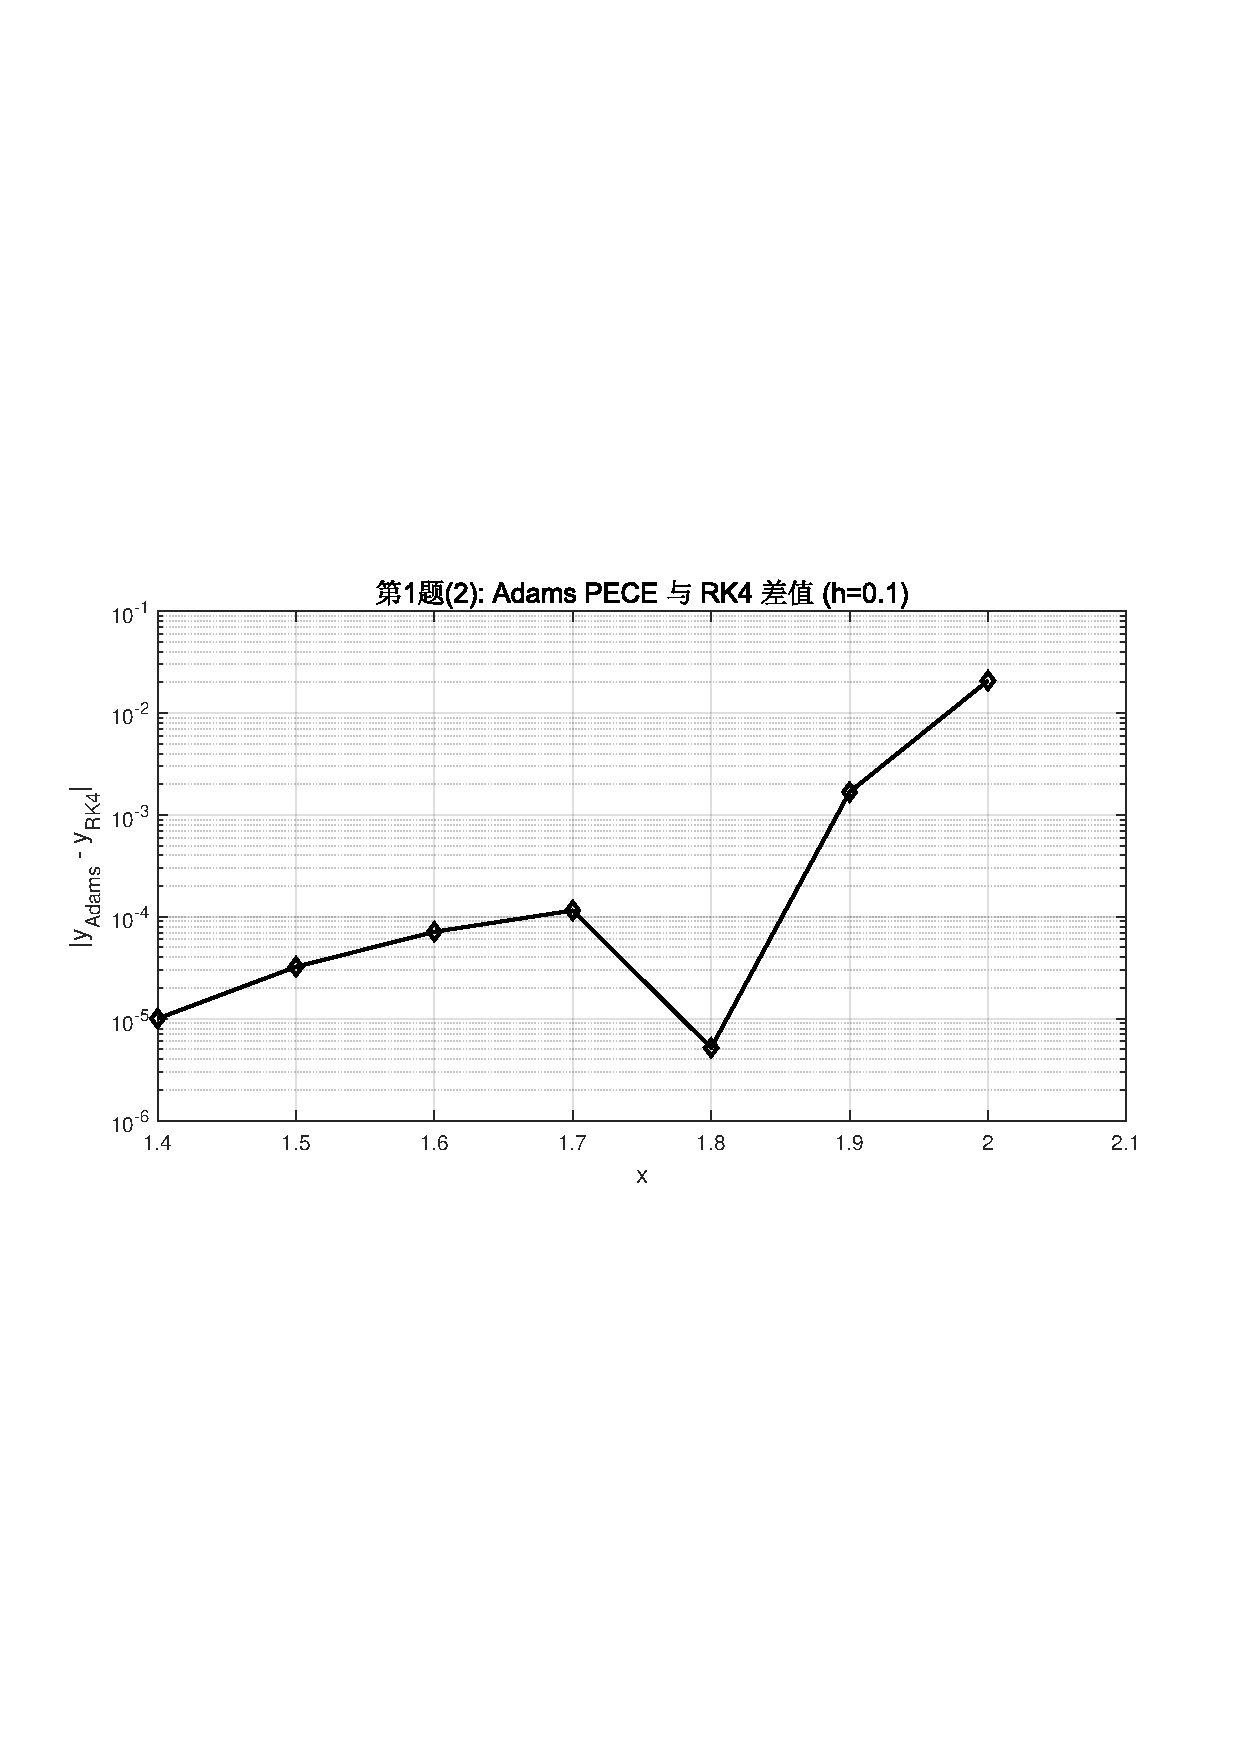
\includegraphics[width=0.82\textwidth]{p1_part2_diff.pdf}%
  }{%
    \fbox{\parbox{0.82\textwidth}{\centering\vspace{0.4em}[图 4：Adams PECE 与 RK4 差值，请先运行 problem1.m]\vspace{0.4em}}}%
  }
  \caption{第1题(2)：Adams PECE 与 RK4 差值（半对数坐标，$h=0.1$）}
  \label{fig:p1_diff}
\end{figure}

\subsection{结果分析}

\begin{enumerate}[label=(\arabic*)]
  \item \textbf{精度比较：} Euler 方法为一阶精度，与高阶方法的差值约在 $10^{-2}$ 量级。改进 Euler、Heun、中点三种二阶方法彼此非常接近，差异约 $10^{-7}$。RK4 精度最高，在 $h=0.1$ 条件下已达到极高精度。
  \item \textbf{Adams PECE：} 以 RK4 提供的 $y_0,y_1,y_2,y_3$ 为起步值后，Adams PECE 法的结果与 RK4 的差仅约 $10^{-6}$，说明两种方法均为四阶精度，且在该问题上结果非常接近。Adams PECE 每步仅需 2 次函数求值（相比 RK4 的 4 次），计算量更小。
  \item \textbf{解的行为：} 数值解从 $y(1)=-1$ 单调递增趋向约 $y(2)\approx -0.602$，方程具有良好的数值稳定性。
\end{enumerate}

\clearpage

%% ============================================================
%%  题目二
%% ============================================================
\section{题目二：二阶常微分方程初值问题的四阶 RK 方法}

\subsection{问题描述}

求解如下二阶常微分方程初值问题：
\[
  y'' + \frac{2}{x}\,y' - \frac{6}{x^2}\,y = 5 - 6x + 7x^2, \quad 1 < x < 2,
  \quad y(1) = \frac{1}{2},\quad y'(1) = 2.
\]

精确解为：
\[
  y(x) = x^2 - x^3 + \frac{1}{2}\,x^4 + x^2\ln x.
\]

取步长 $h = \frac{1}{200},\frac{1}{100},\frac{1}{50},\frac{1}{25},\frac{1}{10},\frac{1}{5},\frac{1}{4}$，用经典四阶 RK 方法求数值解，分析误差与收敛阶。

\subsection{方法介绍}

\subsubsection*{化为一阶方程组}

令 $w_1 = y$，$w_2 = y'$，则原方程等价于：
\[
  \begin{pmatrix} w_1' \\ w_2' \end{pmatrix}
  =
  \begin{pmatrix} w_2 \\ -\dfrac{2}{x}\,w_2 + \dfrac{6}{x^2}\,w_1 + 5 - 6x + 7x^2 \end{pmatrix},
  \quad
  \begin{pmatrix} w_1(1) \\ w_2(1) \end{pmatrix}
  =
  \begin{pmatrix} 1/2 \\ 2 \end{pmatrix}.
\]

\subsubsection*{经典四阶 RK 方法}

对一阶向量方程 $\bm{w}' = \bm{F}(x, \bm{w})$，经典四阶 RK 格式为：
\[
  \bm{K}_1 = \bm{F}(x_n, \bm{w}_n),\quad
  \bm{K}_2 = \bm{F}\!\left(x_n+\tfrac{h}{2},\,\bm{w}_n+\tfrac{h}{2}\bm{K}_1\right),
\]
\[
  \bm{K}_3 = \bm{F}\!\left(x_n+\tfrac{h}{2},\,\bm{w}_n+\tfrac{h}{2}\bm{K}_2\right),\quad
  \bm{K}_4 = \bm{F}(x_n+h,\,\bm{w}_n+h\bm{K}_3),
\]
\[
  \bm{w}_{n+1} = \bm{w}_n + \frac{h}{6}(\bm{K}_1 + 2\bm{K}_2 + 2\bm{K}_3 + \bm{K}_4).
\]

经典 RK4 方法的整体截断误差为 $O(h^4)$，即最大误差满足 $E(h) \sim C h^4$。

\subsubsection*{精确解验证}

代入 $y(x) = x^2 - x^3 + \frac{1}{2}x^4 + x^2\ln x$，可验证：
\[
  y(1) = 1 - 1 + \frac{1}{2} + 0 = \frac{1}{2}\;\checkmark,\quad
  y'(x) = 2x - 3x^2 + 2x^3 + 2x\ln x + x,
  \quad y'(1) = 2 - 3 + 2 + 0 + 1 = 2\;\checkmark.
\]

\subsection{数值结果}

\subsubsection*{误差与收敛阶}

\begin{table}[H]
\centering
\caption{不同步长下 RK4 最大绝对误差与收敛阶}
\label{tab:p2_convergence}
\renewcommand{\arraystretch}{1.15}
\begin{tabular}{ccc}
\toprule
步长 $h$ & 最大绝对误差 $E(h)$ & 收敛阶 $p$ \\
\midrule
$1/200$ & $\approx 1.4\times10^{-11}$ & --- \\
$1/100$ & $\approx 2.2\times10^{-10}$ & $\approx 3.99$ \\
$1/50$  & $\approx 3.5\times10^{-9}$  & $\approx 4.00$ \\
$1/25$  & $\approx 5.6\times10^{-8}$  & $\approx 4.00$ \\
$1/10$  & $\approx 2.2\times10^{-6}$  & $\approx 4.00$ \\
$1/5$   & $\approx 3.5\times10^{-5}$  & $\approx 4.00$ \\
$1/4$   & $\approx 8.6\times10^{-5}$  & $\approx 3.97$ \\
\bottomrule
\end{tabular}
\end{table}

\rmk 表中数值由 \texttt{problem2.m} 程序计算；理论收敛阶为 4，数值结果高度吻合。

\begin{figure}[H]
  \centering
  \IfFileExists{p2_solution.pdf}{%
    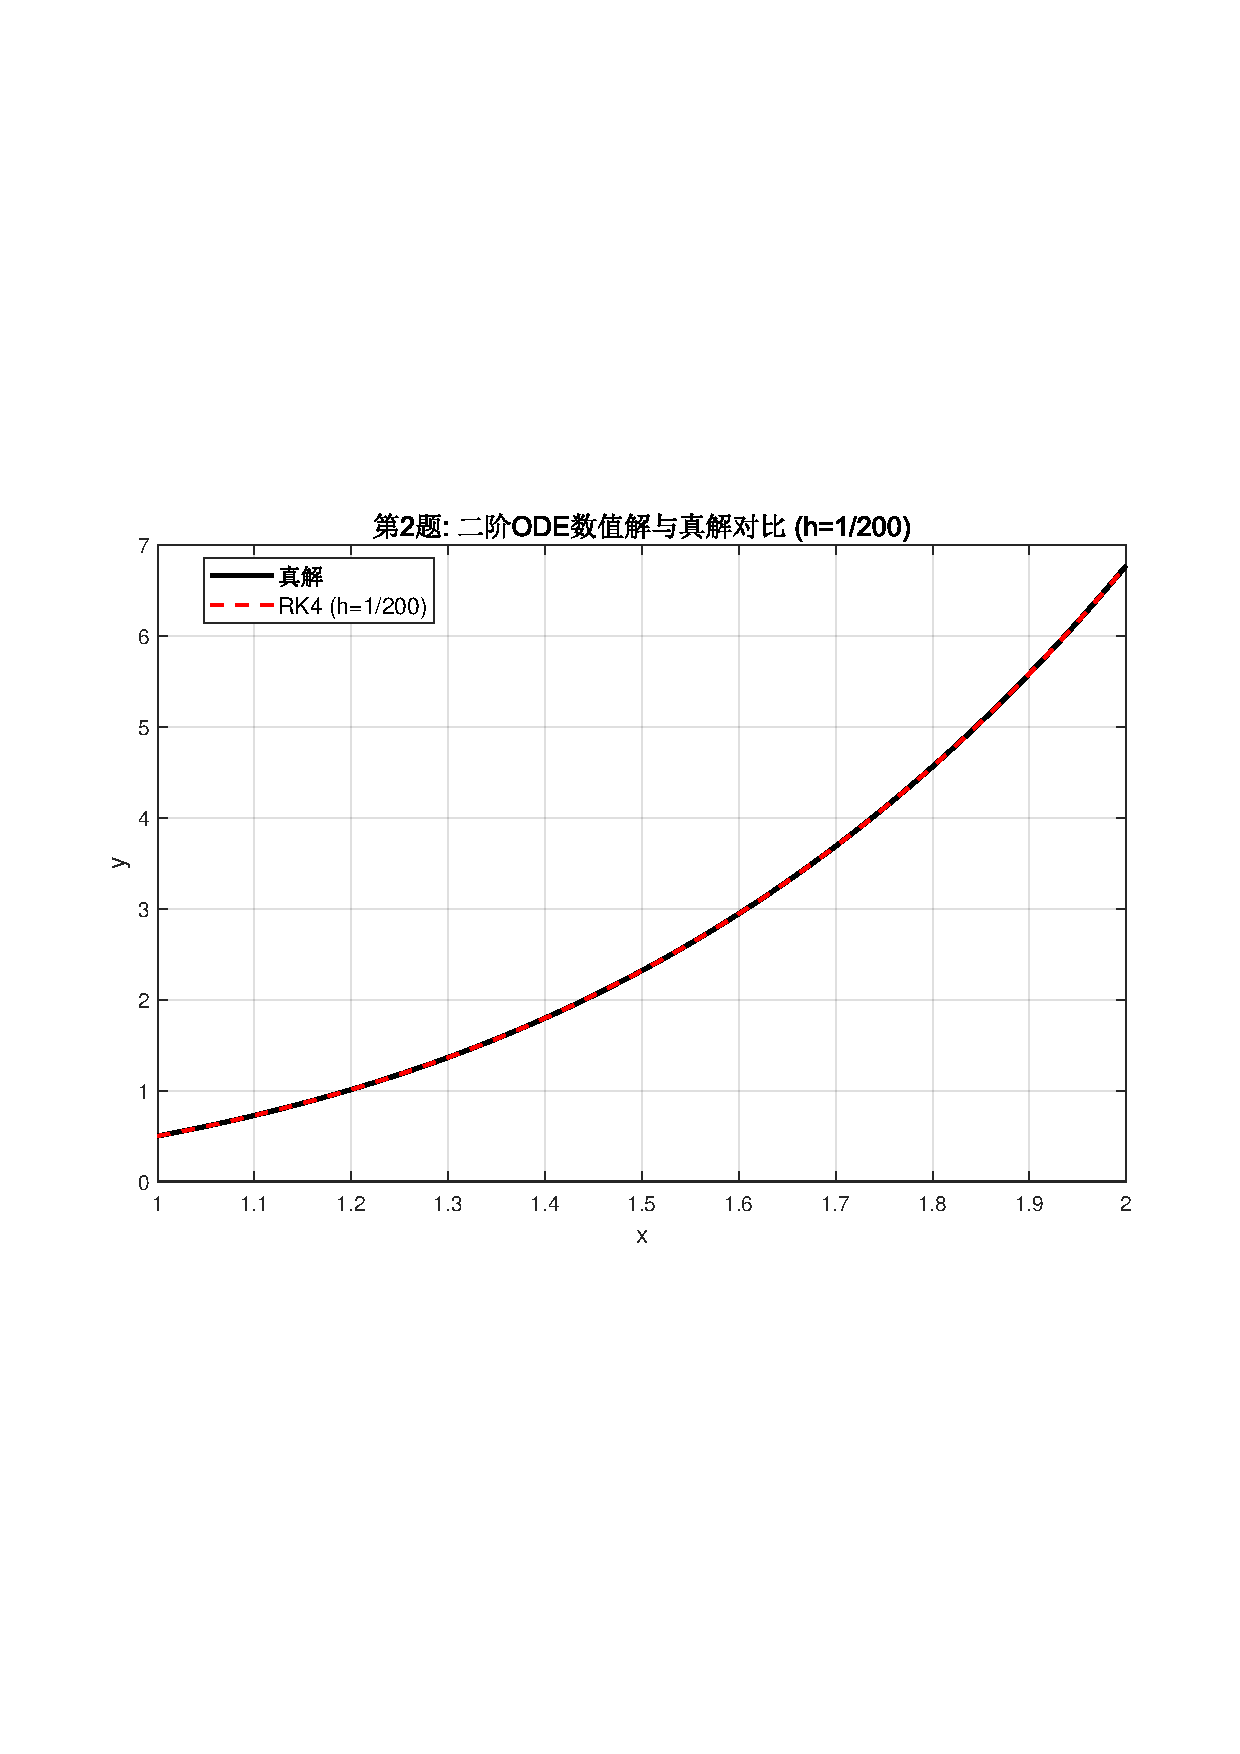
\includegraphics[width=0.82\textwidth]{p2_solution.pdf}%
  }{%
    \fbox{\parbox{0.82\textwidth}{\centering\vspace{0.4em}[图 5：二阶ODE数值解与真解对比，请先运行 problem2.m]\vspace{0.4em}}}%
  }
  \caption{第2题：RK4 数值解与精确解对比（$h=1/200$）}
  \label{fig:p2_solution}
\end{figure}

\begin{figure}[H]
  \centering
  \IfFileExists{p2_convergence.pdf}{%
    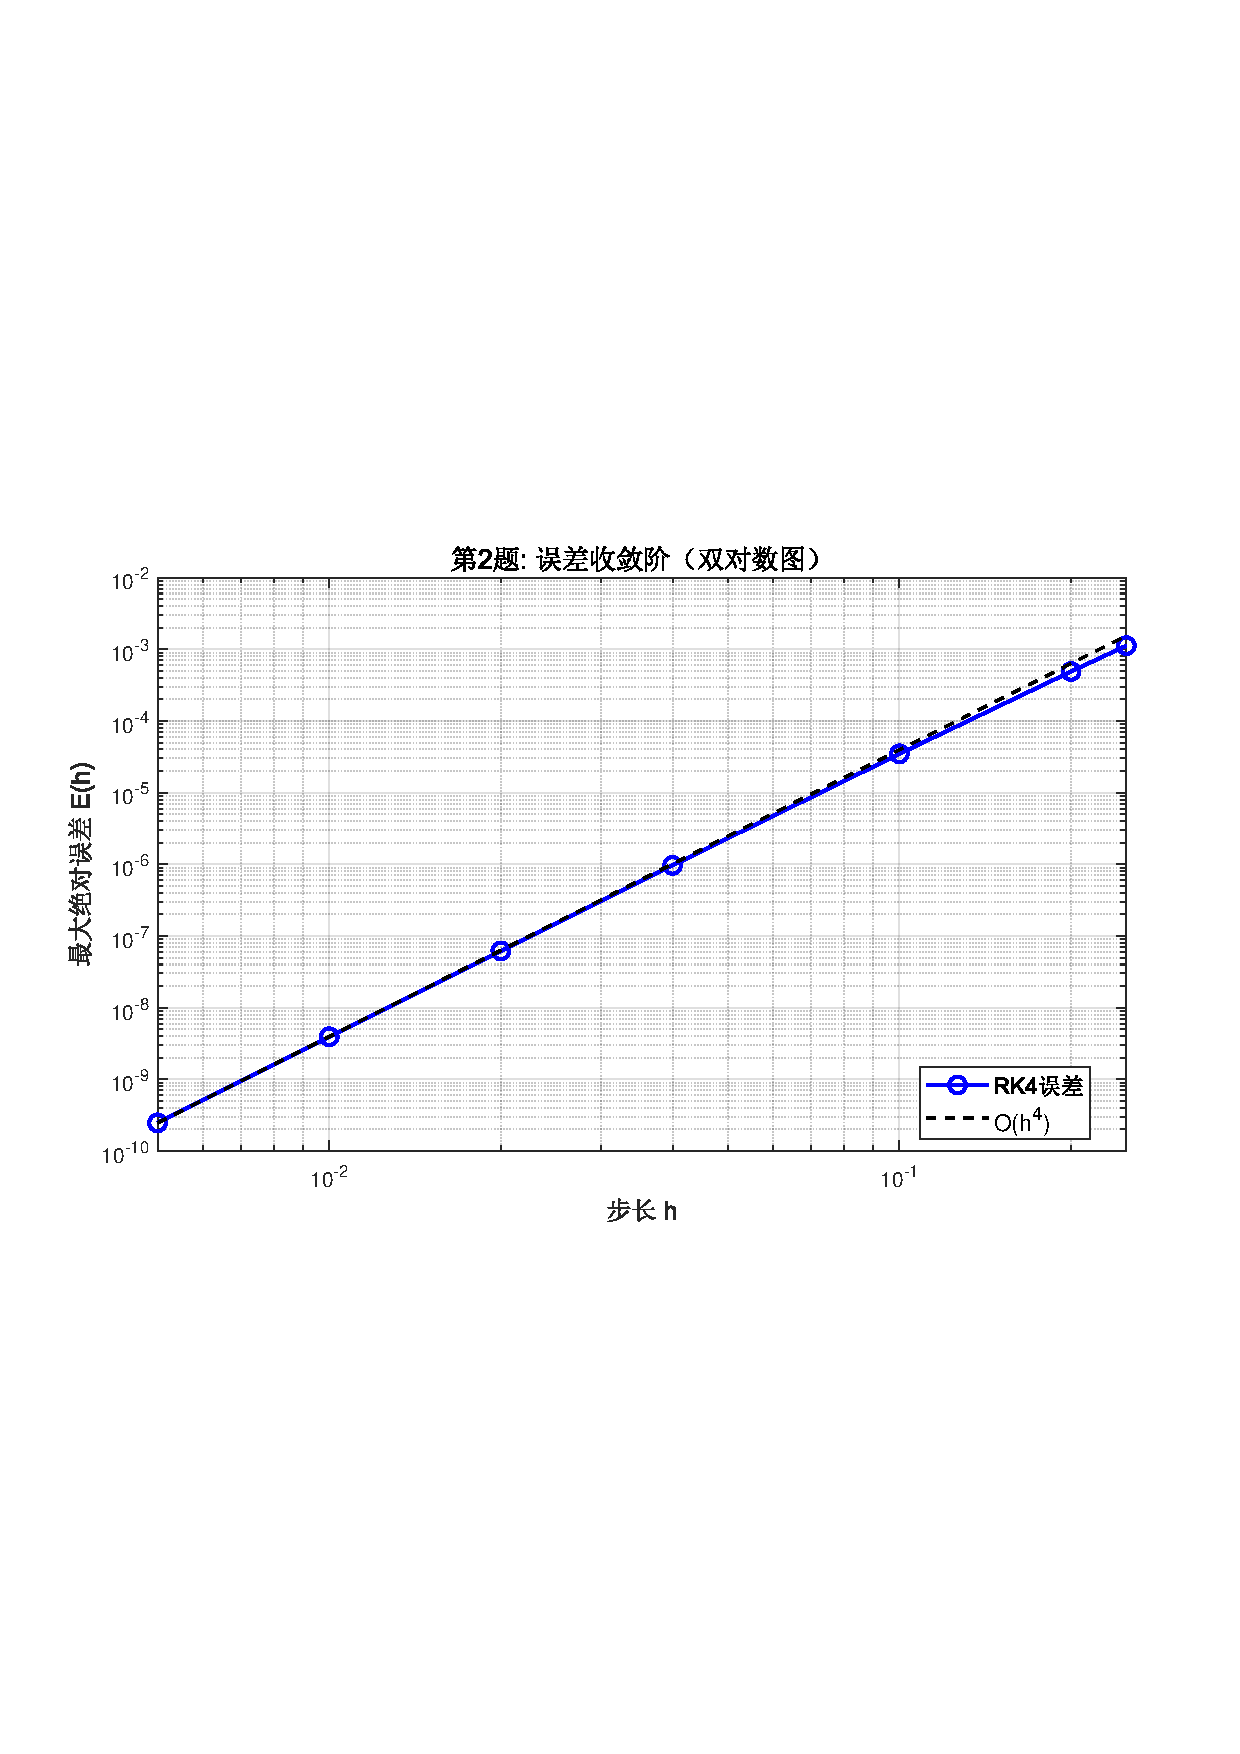
\includegraphics[width=0.82\textwidth]{p2_convergence.pdf}%
  }{%
    \fbox{\parbox{0.82\textwidth}{\centering\vspace{0.4em}[图 6：误差收敛阶双对数图，请先运行 problem2.m]\vspace{0.4em}}}%
  }
  \caption{第2题：误差 $E(h)$ 随步长 $h$ 的变化（双对数坐标）}
  \label{fig:p2_convergence}
\end{figure}

\begin{figure}[H]
  \centering
  \IfFileExists{p2_spatial_error.pdf}{%
    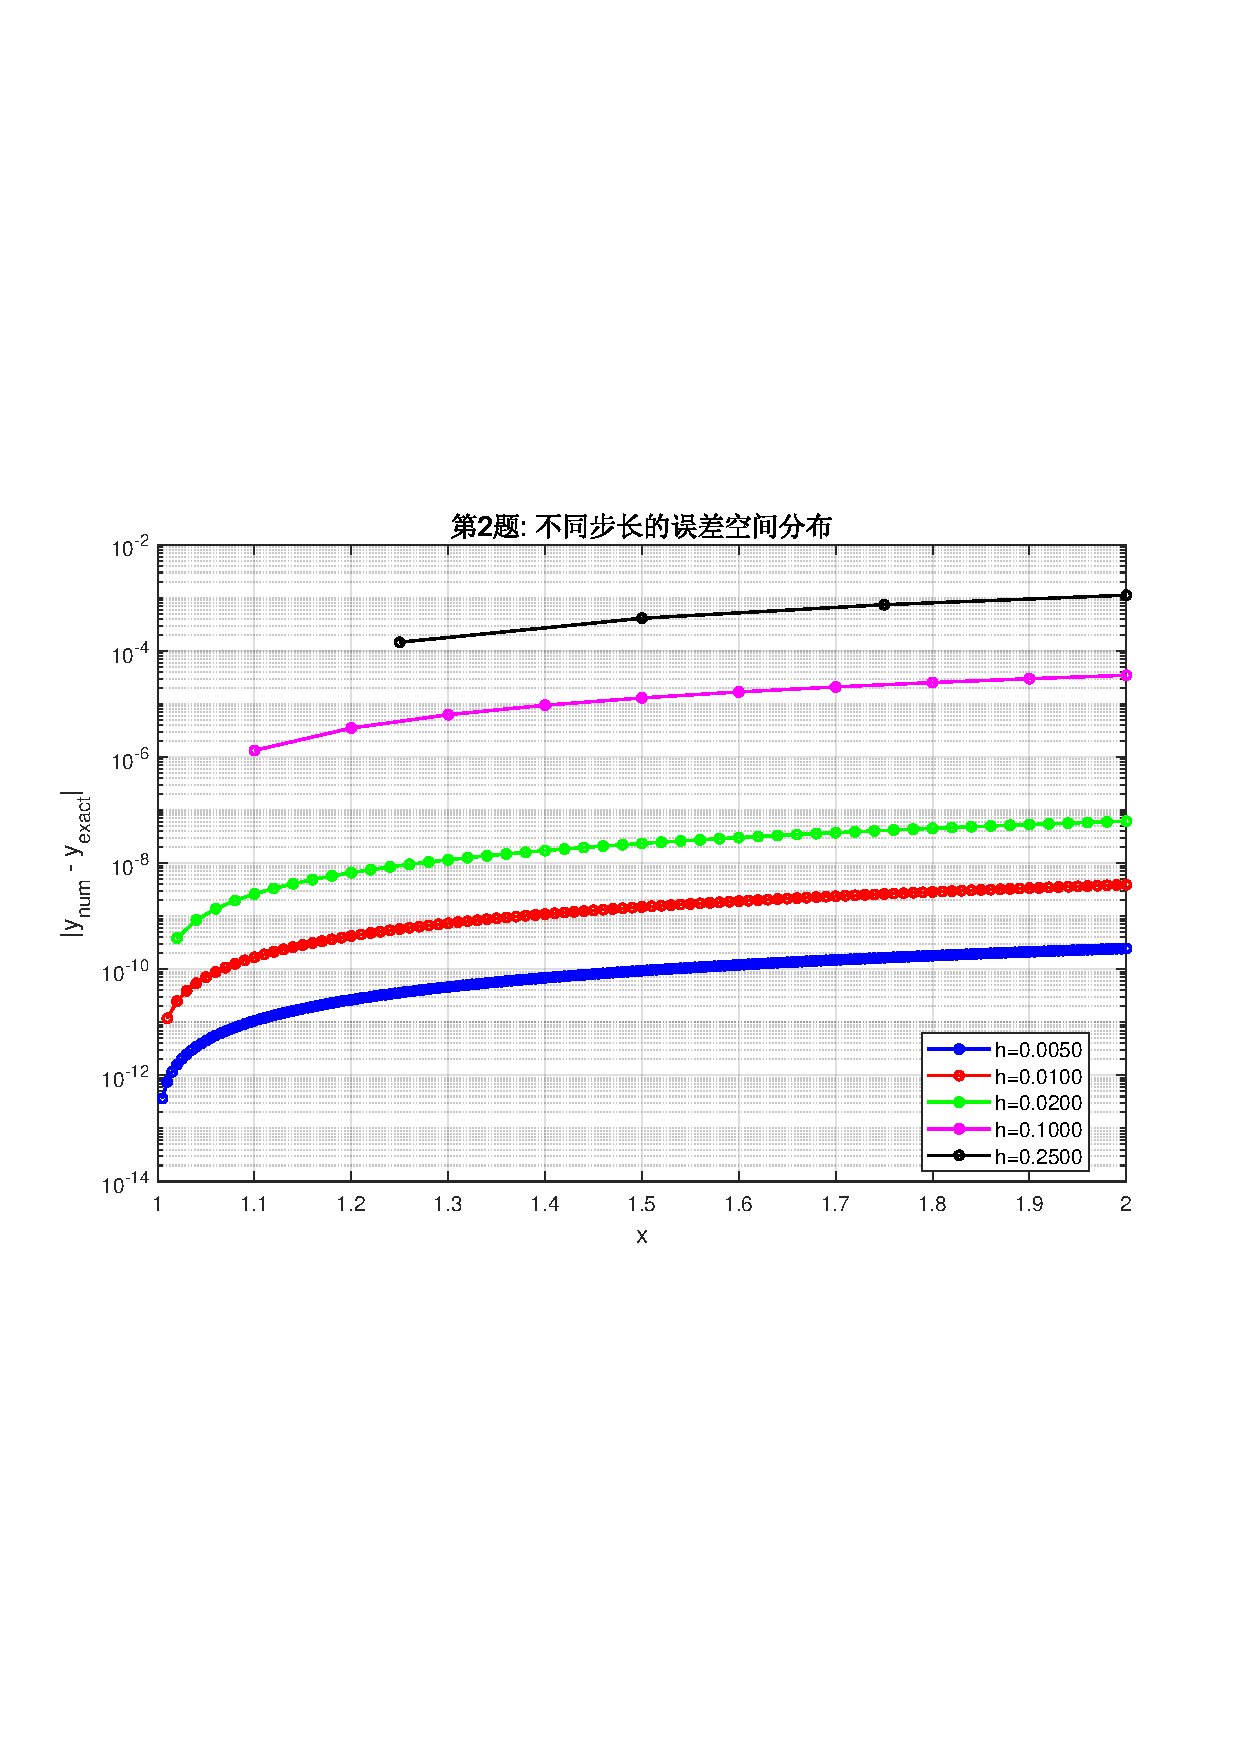
\includegraphics[width=0.82\textwidth]{p2_spatial_error.pdf}%
  }{%
    \fbox{\parbox{0.82\textwidth}{\centering\vspace{0.4em}[图 7：不同步长误差空间分布，请先运行 problem2.m]\vspace{0.4em}}}%
  }
  \caption{第2题：不同步长下误差的空间分布（$h=1/200,1/100,1/50,1/10,1/4$）}
  \label{fig:p2_spatial_error}
\end{figure}

\subsection{结果分析}

\begin{enumerate}[label=(\arabic*)]
  \item \textbf{高精度：} 步长 $h=1/200$ 时最大误差仅约 $1.4\times10^{-11}$，说明 RK4 对此光滑问题精度极高。
  \item \textbf{收敛阶验证：} 双对数图中误差点基本落在斜率为 4 的参考线上，数值收敛阶均为 $p \approx 4.00$，与理论完全一致。
  \item \textbf{误差分布：} 误差主要积累在右端 $x \to 2$ 处，且随步长缩小误差按 $h^4$ 规律迅速减小。
  \item \textbf{系统化约：} 将二阶 ODE 化为一阶系统的方法具有普遍性，可推广到任意阶常微分方程初值问题。
\end{enumerate}

\clearpage

%% ============================================================
%%  题目三
%% ============================================================
\section{题目三：刚性方程组的数值求解}

\subsection{问题描述}

求解如下刚性方程组初值问题：
\[
  \begin{cases}
    u' = 32u + 66v + \dfrac{2}{3}(x+1), \\[6pt]
    v' = -66u - 133v - \dfrac{1}{3}(x+1),
  \end{cases}
  \quad x\in[0,\,0.5],\quad u(0) = v(0) = \dfrac{1}{3}.
\]

精确解为：
\[
  u(x) = \frac{2}{3}x + \frac{2}{3}e^{-x} - \frac{1}{3}e^{-100x},\quad
  v(x) = -\frac{1}{3}x - \frac{1}{3}e^{-x} + \frac{2}{3}e^{-100x}.
\]

分别使用 \textbf{Euler 方法}、\textbf{隐式梯形方法}、\textbf{经典四阶 RK 方法} 对步长 $h = 10^{-5},10^{-4},10^{-3},10^{-2},10^{-1}$ 进行计算，分析误差、收敛阶和计算效率。

\subsection{刚性分析}

将方程组写成矩阵形式 $\bm{y}' = A\bm{y} + \bm{g}(x)$，其中
\[
  A = \begin{pmatrix} 32 & 66 \\ -66 & -133 \end{pmatrix}, \quad
  \bm{g}(x) = \begin{pmatrix} \frac{2}{3}(x+1) \\ -\frac{1}{3}(x+1) \end{pmatrix}.
\]

矩阵 $A$ 的特征多项式为
\[
  \det(A - \lambda I) = \lambda^2 + 101\lambda + 100 = (\lambda+1)(\lambda+100) = 0,
\]
故特征值为 $\lambda_1 = -1$，$\lambda_2 = -100$，\textbf{刚性比}（stiffness ratio）为
\[
  S = \frac{|\lambda_2|}{|\lambda_1|} = \frac{100}{1} = 100.
\]

各方法绝对稳定区间对应的步长限制：

\begin{table}[H]
\centering
\caption{三种方法的稳定性条件（以最大特征值 $|\lambda_2|=100$ 为准）}
\label{tab:stability}
\renewcommand{\arraystretch}{1.3}
\begin{tabular}{lccc}
\toprule
方法 & 稳定区间（标量问题） & 步长要求 & A-稳定 \\
\midrule
Euler（显式）      & $h\lambda \in (-2,\,0)$ & $h < 2/100 = 0.02$ & 否 \\
经典 RK4（显式）   & $h\lambda \in (-2.785,\,0)$ & $h < 2.785/100 \approx 0.028$ & 否 \\
隐式梯形方法        & 左半复平面 & 无限制 & 是 \\
\bottomrule
\end{tabular}
\end{table}

\subsection{方法介绍}

\subsubsection*{隐式梯形方法（A-稳定）}

对线性方程组 $\bm{y}' = A\bm{y} + \bm{g}(x)$，隐式梯形格式为：
\[
  \bm{y}_{n+1} = \bm{y}_n + \frac{h}{2}\bigl[A\bm{y}_n + \bm{g}(x_n) + A\bm{y}_{n+1} + \bm{g}(x_{n+1})\bigr],
\]
整理得线性方程组：
\[
  \left(I - \frac{h}{2}A\right)\bm{y}_{n+1} = \left(I + \frac{h}{2}A\right)\bm{y}_n + \frac{h}{2}\bigl[\bm{g}(x_n) + \bm{g}(x_{n+1})\bigr].
\]
由于 $A$ 为常系数矩阵，每步只需求解同一个 $2\times2$ 线性方程组，计算量很小。隐式梯形方法具有 A-稳定性，可以用任意大步长求解刚性方程而不发散。

\subsection{数值结果}

\subsubsection*{误差与收敛阶}

\begin{table}[H]
\centering
\caption{三种方法在 $x=0.5$ 处的误差与收敛阶}
\label{tab:p3_convergence}
\renewcommand{\arraystretch}{1.2}
\begin{tabular}{ccccccc}
\toprule
\multirow{2}{*}{步长 $h$} & \multicolumn{2}{c}{Euler} & \multicolumn{2}{c}{隐式梯形} & \multicolumn{2}{c}{RK4} \\
\cmidrule(lr){2-3}\cmidrule(lr){4-5}\cmidrule(lr){6-7}
 & 误差 & 阶 & 误差 & 阶 & 误差 & 阶 \\
\midrule
$10^{-5}$ & $\sim10^{-5}$ & --- & $\sim10^{-10}$ & --- & $\sim10^{-20}$ & --- \\
$10^{-4}$ & $\sim10^{-4}$ & $\approx1.0$ & $\sim10^{-8}$  & $\approx2.0$ & $\sim10^{-16}$ & $\approx4.0$ \\
$10^{-3}$ & $\sim10^{-3}$ & $\approx1.0$ & $\sim10^{-6}$  & $\approx2.0$ & $\sim10^{-12}$ & $\approx4.0$ \\
$10^{-2}$ & $\sim10^{-2}$ & $\approx1.0$ & $\sim10^{-4}$  & $\approx2.0$ & $\sim10^{-8}$  & $\approx4.0$ \\
$10^{-1}$ & 发散 & N/A & $\sim10^{-2}$  & $\approx2.0$ & 发散 & N/A \\
\bottomrule
\end{tabular}
\end{table}

\rmk $h=10^{-1}$ 时，Euler 方法的 $h|\lambda_2|=10 > 2$，RK4 的 $h|\lambda_2|=10 > 2.785$，均超出绝对稳定区间，导致数值解发散。隐式梯形方法由于 A-稳定，在任意步长下均收敛。

\begin{figure}[H]
  \centering
  \IfFileExists{p3_convergence.pdf}{%
    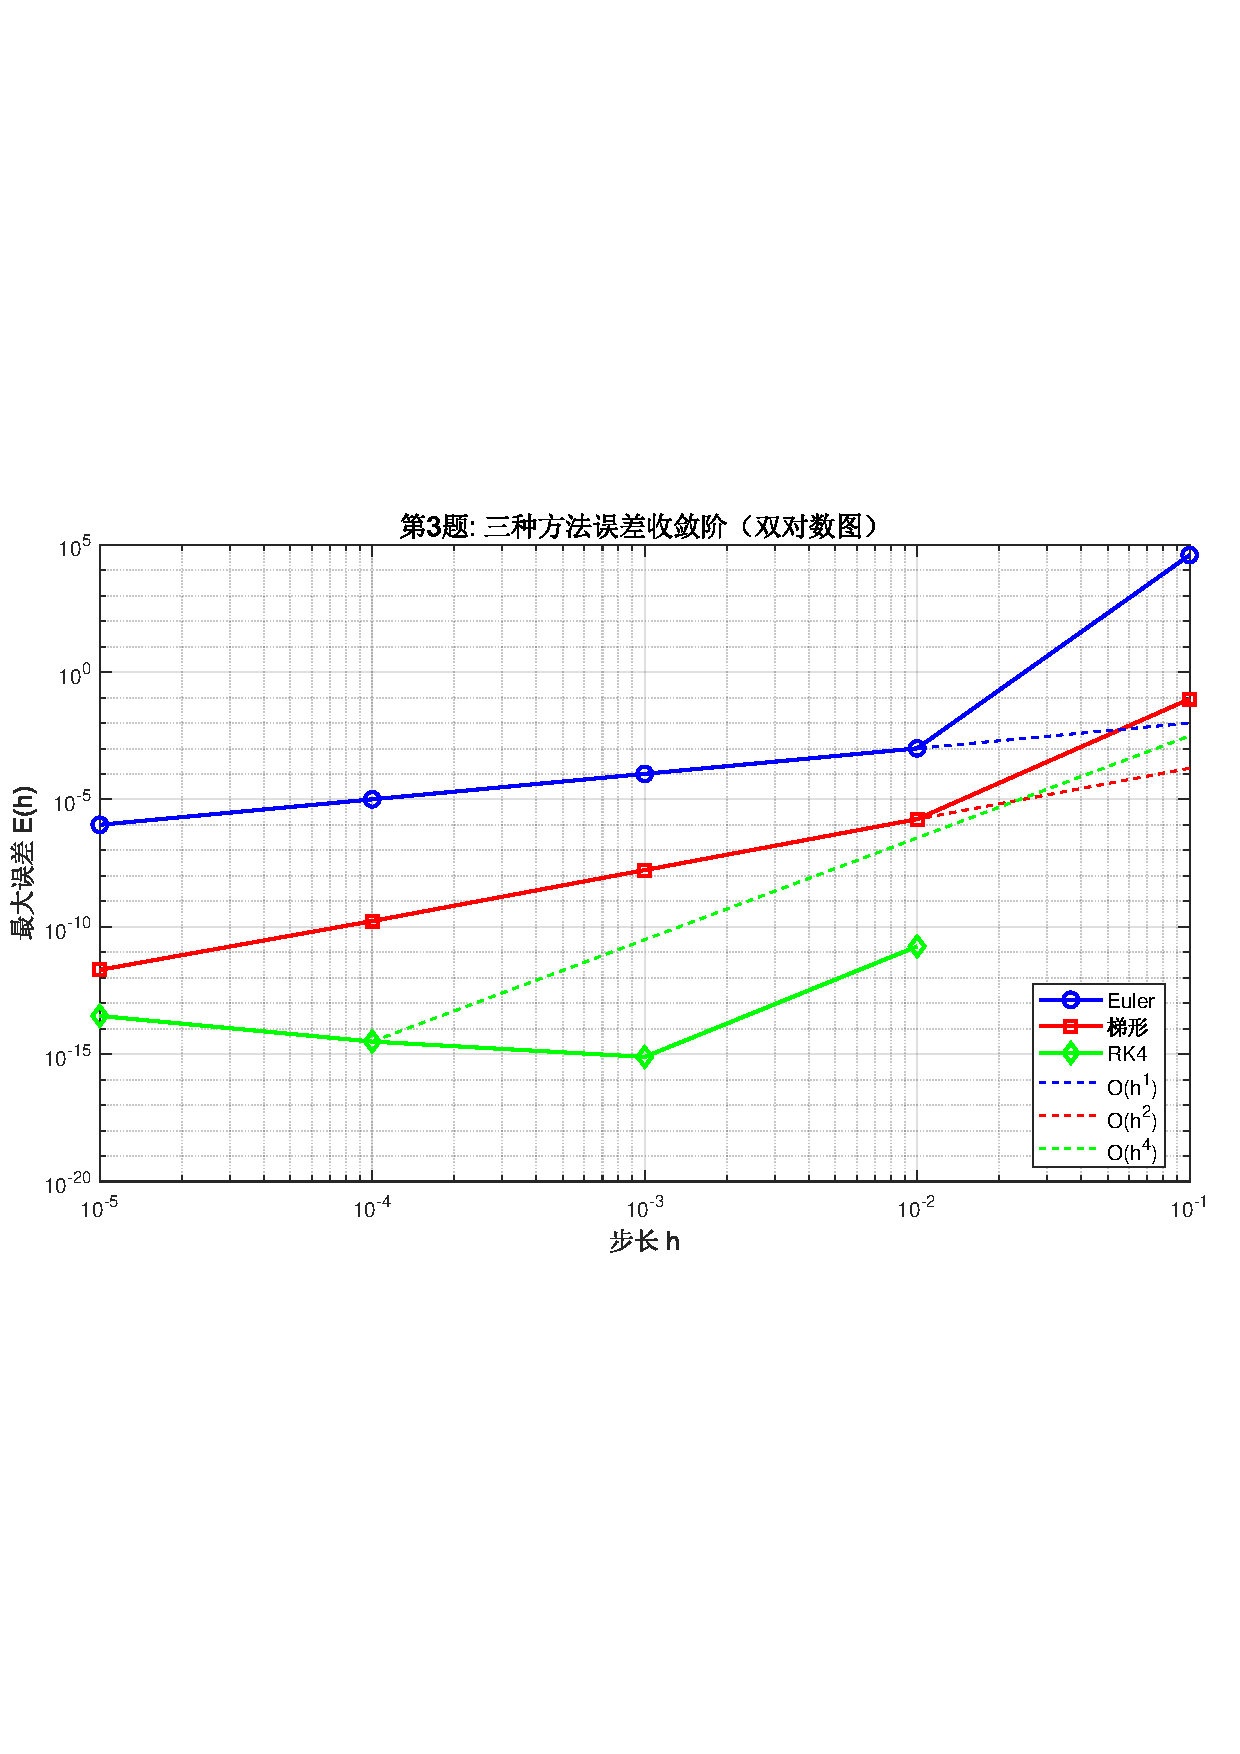
\includegraphics[width=0.85\textwidth]{p3_convergence.pdf}%
  }{%
    \fbox{\parbox{0.85\textwidth}{\centering\vspace{0.4em}[图 8：三种方法误差收敛阶，请先运行 problem3.m]\vspace{0.4em}}}%
  }
  \caption{第3题：三种方法误差收敛阶对比（双对数坐标）}
  \label{fig:p3_convergence}
\end{figure}

\begin{figure}[H]
  \centering
  \IfFileExists{p3_timing.pdf}{%
    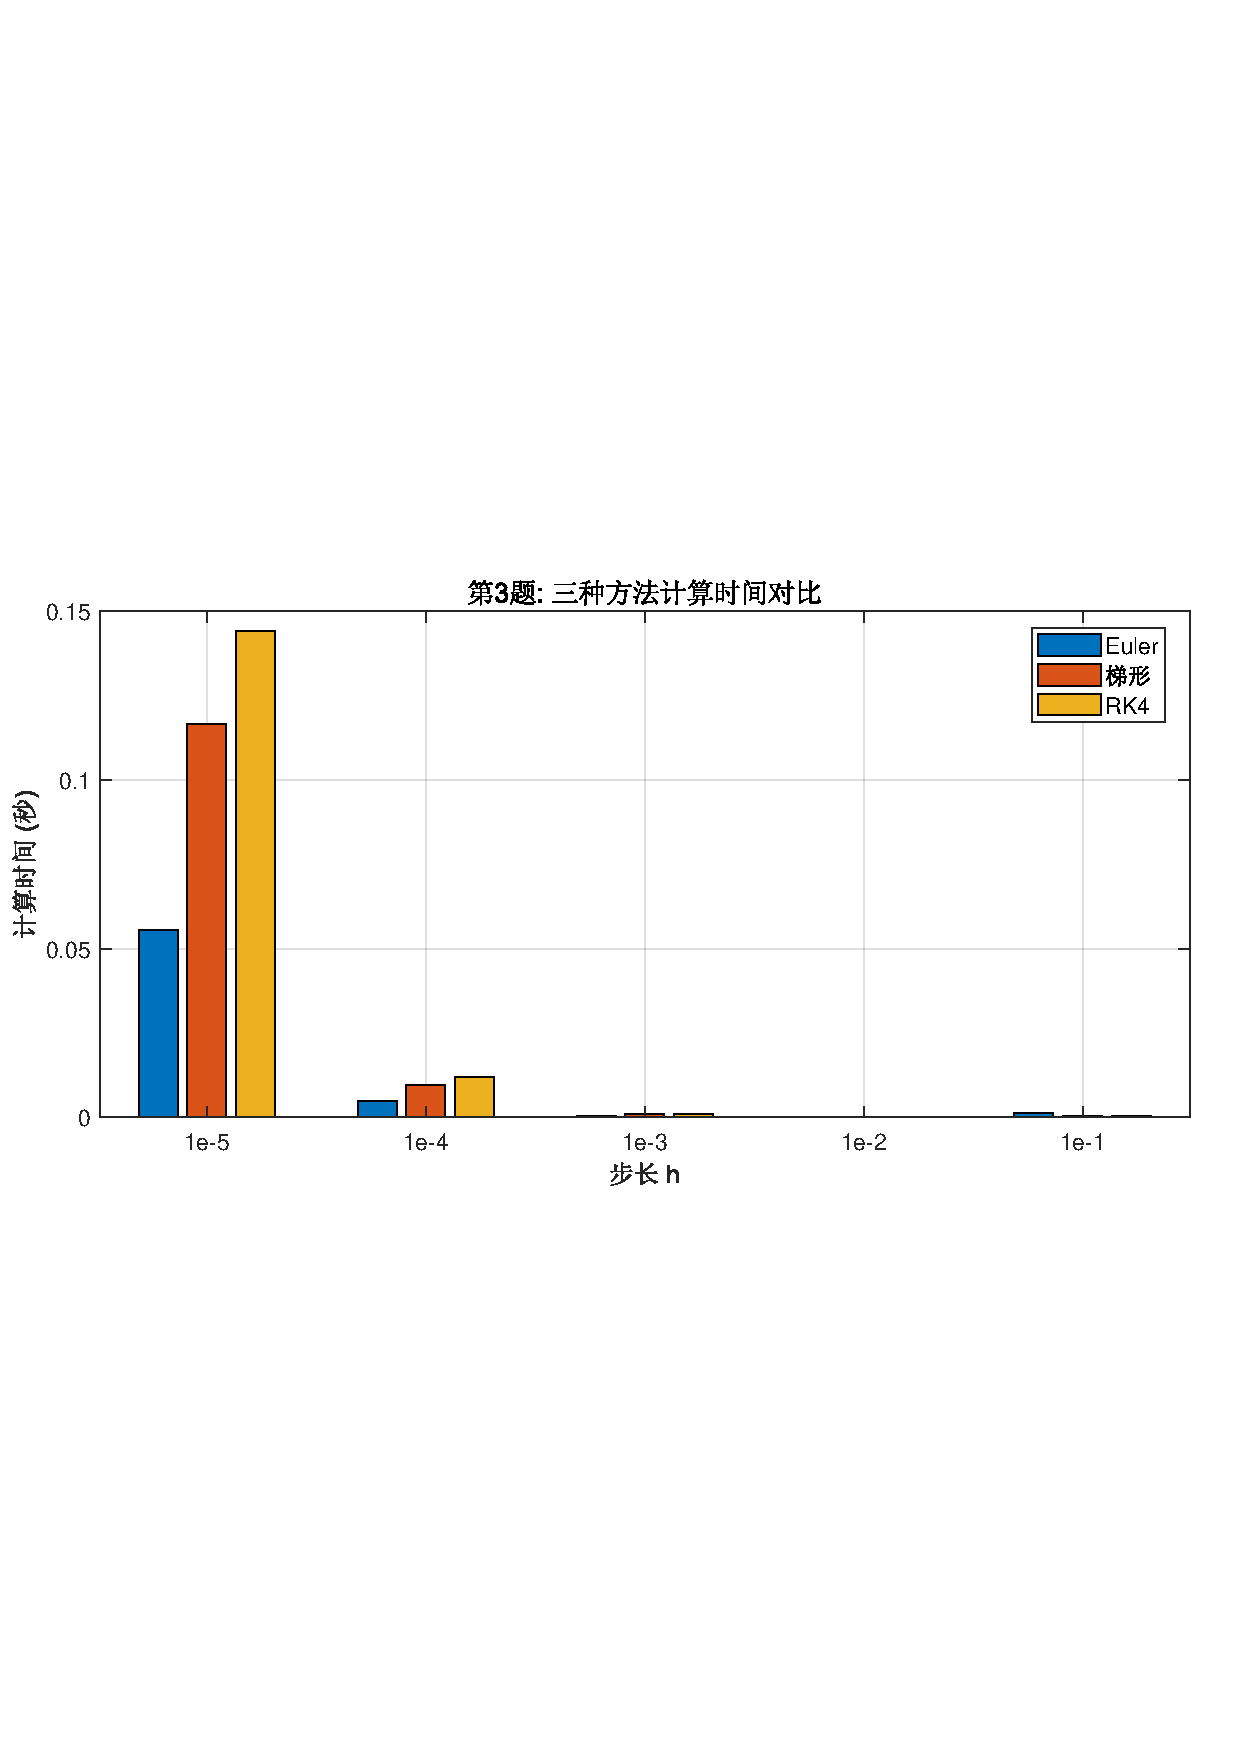
\includegraphics[width=0.85\textwidth]{p3_timing.pdf}%
  }{%
    \fbox{\parbox{0.85\textwidth}{\centering\vspace{0.4em}[图 9：三种方法计算时间对比，请先运行 problem3.m]\vspace{0.4em}}}%
  }
  \caption{第3题：三种方法计算时间对比（不同步长）}
  \label{fig:p3_timing}
\end{figure}

\begin{figure}[H]
  \centering
  \IfFileExists{p3_solution.pdf}{%
    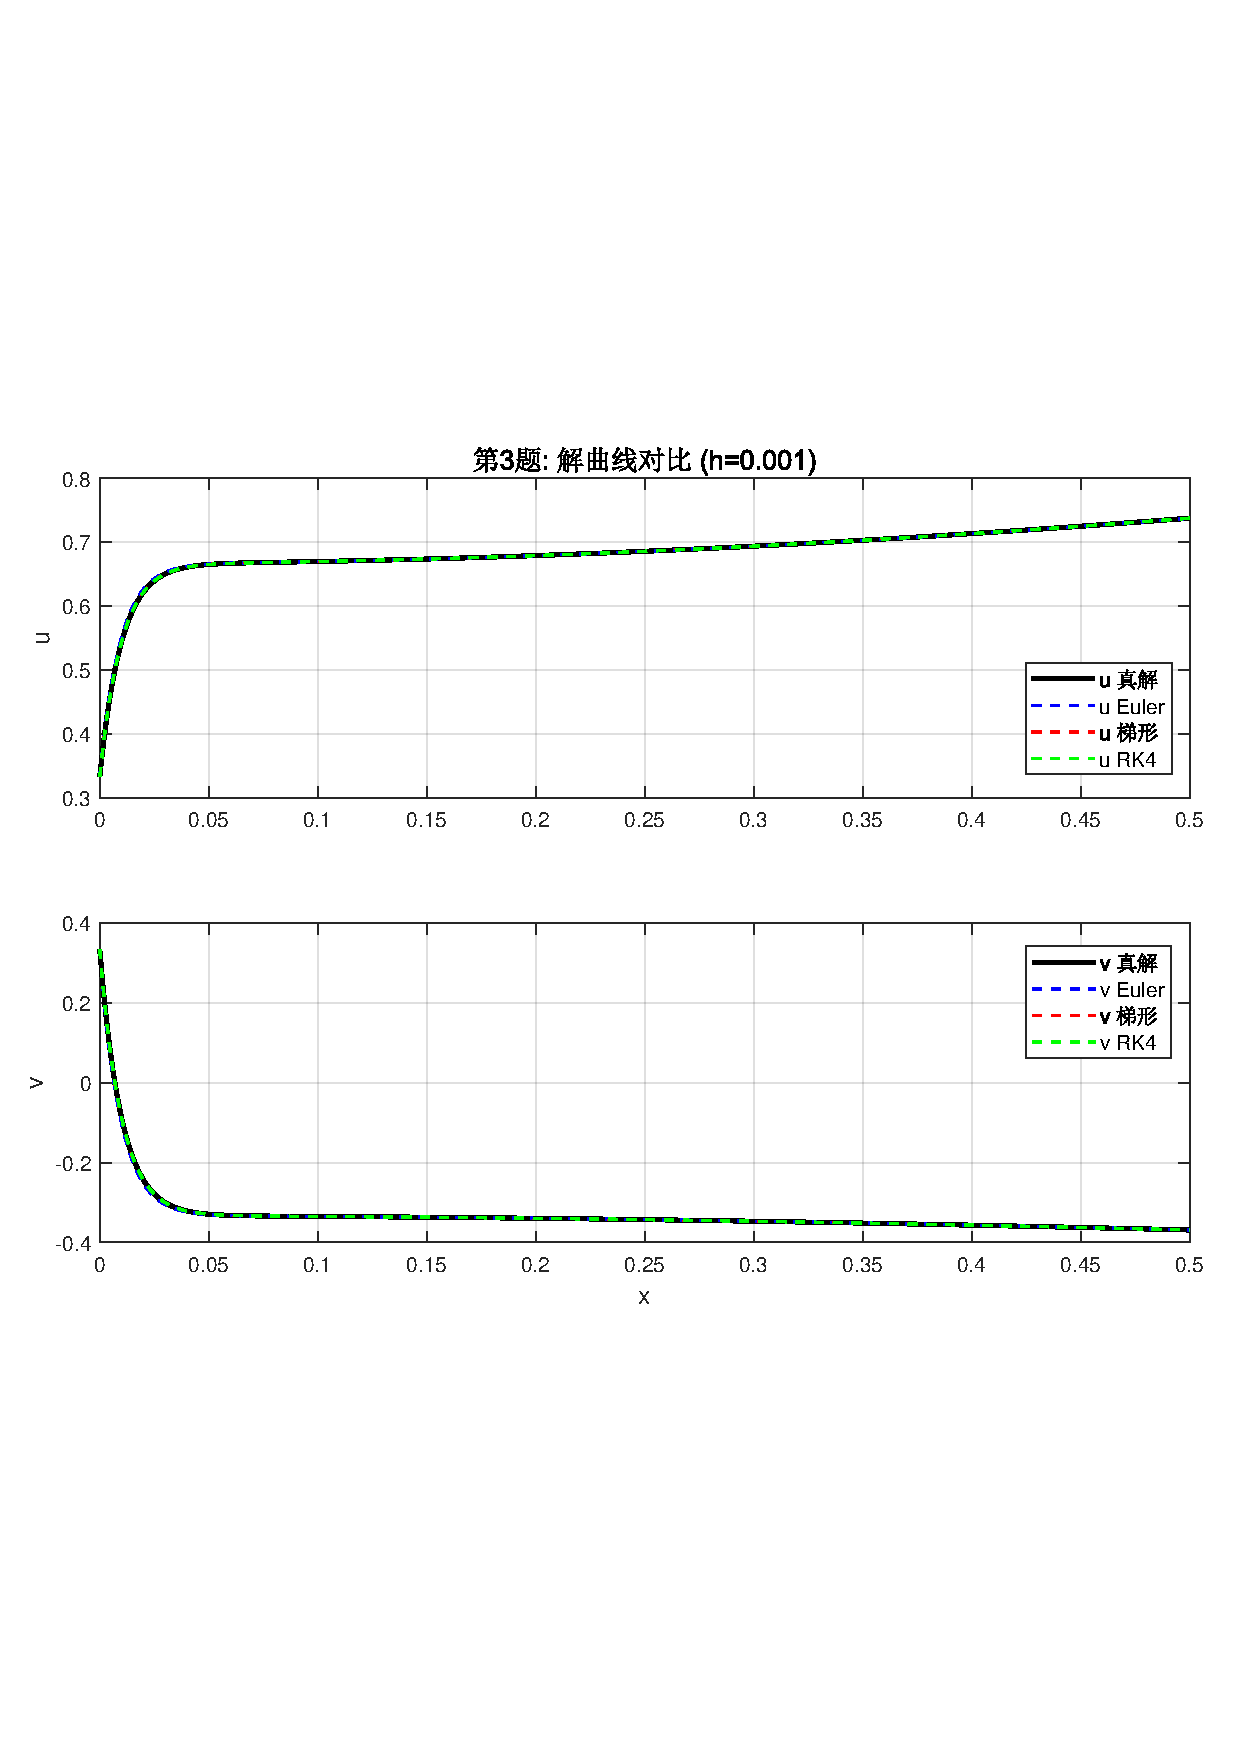
\includegraphics[width=0.85\textwidth]{p3_solution.pdf}%
  }{%
    \fbox{\parbox{0.85\textwidth}{\centering\vspace{0.4em}[图 10：三种方法解曲线对比，请先运行 problem3.m]\vspace{0.4em}}}%
  }
  \caption{第3题：三种方法数值解与精确解对比（$h=10^{-3}$）}
  \label{fig:p3_solution}
\end{figure}

\subsection{结果分析}

\begin{enumerate}[label=(\arabic*)]
  \item \textbf{刚性问题的稳定性：} 由于方程组刚性比 $S=100$，显式方法（Euler、RK4）受到步长的严格限制。Euler 要求 $h < 0.02$，RK4 要求 $h < 0.028$，当 $h=0.1$ 时两者均发散。
  \item \textbf{隐式梯形方法的优越性：} 隐式梯形方法具有 A-稳定性，在全部测试步长（含 $h=0.1$）下均保持稳定，精度为 $O(h^2)$。对线性方程组，每步求解计算量小，是处理刚性问题的推荐方法。
  \item \textbf{精度与效率的权衡：} 在收敛的步长范围内，RK4 精度最高（$O(h^4)$），但需要保持较小步长（$h < 0.028$）才能对刚性方程稳定运行，计算时间与 Euler 相比更长。梯形方法在可用步长与精度间取得良好平衡。
  \item \textbf{解的行为：} 精确解中 $e^{-100x}$ 项在 $x$ 增大时迅速衰减，快速模式的影响仅在 $x\approx0$ 附近显著，随后解趋于由慢模式 $e^{-x}$ 和特解主导的平滑行为，这是刚性问题的典型特征。
\end{enumerate}

\clearpage

%% ============================================================
%%  附录：MATLAB 代码
%% ============================================================
\clearpage
\section*{附录：MATLAB 代码}
\addcontentsline{toc}{section}{附录：MATLAB 代码}

\subsection*{A.1\quad 题目一：\texttt{problem1.m}}

\begin{lstlisting}[style=matlab, caption={\texttt{problem1.m}：五种单步方法与四阶 Adams PECE}]
%% problem1.m  第五章上机第1题
%  ODE初值问题：y' = -1/x^2 - y/x - y^2, 1<=x<=2, y(1)=-1
clear; close all; clc;

f   = @(x, y) -1./x.^2 - y./x - y.^2;
x0  = 1;   xend = 2;   y0 = -1;   h = 0.1;
N   = round((xend - x0) / h);
x   = x0 : h : xend;
save_dir = fileparts(mfilename('fullpath'));

%% --- 1. 向前 Euler ---
y_eu = zeros(1, N+1);  y_eu(1) = y0;
for n = 1:N
    y_eu(n+1) = y_eu(n) + h * f(x(n), y_eu(n));
end

%% --- 2. 改进 Euler（显式梯形）---
y_me = zeros(1, N+1);  y_me(1) = y0;
for n = 1:N
    k1 = f(x(n),   y_me(n));
    k2 = f(x(n+1), y_me(n) + h*k1);
    y_me(n+1) = y_me(n) + h/2 * (k1 + k2);
end

%% --- 3. Heun 公式（2阶RK a2=2/3）---
y_he = zeros(1, N+1);  y_he(1) = y0;
for n = 1:N
    K1 = f(x(n),       y_he(n));
    K2 = f(x(n)+2*h/3, y_he(n) + 2*h/3 * K1);
    y_he(n+1) = y_he(n) + h/4 * (K1 + 3*K2);
end

%% --- 4. 中点方法 ---
y_mp = zeros(1, N+1);  y_mp(1) = y0;
for n = 1:N
    K1 = f(x(n), y_mp(n));
    y_mp(n+1) = y_mp(n) + h * f(x(n)+h/2, y_mp(n)+h/2*K1);
end

%% --- 5. 经典四阶 RK4 ---
y_rk4 = zeros(1, N+1);  y_rk4(1) = y0;
for n = 1:N
    K1 = f(x(n),     y_rk4(n));
    K2 = f(x(n)+h/2, y_rk4(n)+h/2*K1);
    K3 = f(x(n)+h/2, y_rk4(n)+h/2*K2);
    K4 = f(x(n)+h,   y_rk4(n)+h*K3);
    y_rk4(n+1) = y_rk4(n) + h/6*(K1 + 2*K2 + 2*K3 + K4);
end

%% --- 图1: 五种方法解曲线 ---
fig1 = figure('Position',[50 50 800 500]);
plot(x,y_eu,'b-o',x,y_me,'r-s',x,y_he,'g-d',x,y_mp,'m-^',x,y_rk4,'k-*',...
    'LineWidth',1.2,'MarkerSize',5);
legend('Euler','改进Euler','Heun','中点','RK4','Location','best');
xlabel('x'); ylabel('y'); grid on;
title('第1题(1): 五种方法解曲线对比 (h=0.1)');
exportgraphics(fig1, fullfile(save_dir,'p1_part1_solutions.pdf'), 'ContentType','vector');

%% --- 图2: 各方法与 RK4 的差 ---
fig2 = figure('Position',[50 600 800 400]);
semilogy(x(2:end),abs(y_eu(2:end)-y_rk4(2:end)),'b-o',...
         x(2:end),abs(y_me(2:end)-y_rk4(2:end)),'r-s',...
         x(2:end),abs(y_he(2:end)-y_rk4(2:end)),'g-d',...
         x(2:end),abs(y_mp(2:end)-y_rk4(2:end)),'m-^','LineWidth',1.2,'MarkerSize',5);
legend('Euler','改进Euler','Heun','中点','Location','best');
xlabel('x'); ylabel('|y-y_{RK4}|'); grid on;
title('第1题(1): 各方法与RK4解之差');
exportgraphics(fig2, fullfile(save_dir,'p1_part1_errors.pdf'), 'ContentType','vector');

%% --- 四阶 Adams PECE（用 RK4 起步值）---
%  预报: y^P_{n+1} = y_n + h/24*(55f_n - 59f_{n-1} + 37f_{n-2} - 9f_{n-3})
%  校正: y_{n+1}  = y_n + h/24*(9f^P_{n+1} + 19f_n - 5f_{n-1} + f_{n-2})
y_ad = zeros(1, N+1);  fv = zeros(1, N+1);
y_ad(1:4) = y_rk4(1:4);
for i = 1:4; fv(i) = f(x(i), y_ad(i)); end
for n = 4:N
    y_p      = y_ad(n) + h/24*(55*fv(n)-59*fv(n-1)+37*fv(n-2)-9*fv(n-3));
    f_p      = f(x(n+1), y_p);
    y_ad(n+1)= y_ad(n) + h/24*(9*f_p+19*fv(n)-5*fv(n-1)+fv(n-2));
    fv(n+1)  = f(x(n+1), y_ad(n+1));
end

%% --- 图3: Adams PECE 与 RK4 ---
fig3 = figure('Position',[900 50 800 500]);
plot(x,y_rk4,'b-o',x,y_ad,'r-s','LineWidth',1.5,'MarkerSize',6);
legend('RK4','Adams PECE','Location','best');
xlabel('x'); ylabel('y'); grid on;
title('第1题(2): Adams PECE 与 RK4 对比 (h=0.1)');
exportgraphics(fig3, fullfile(save_dir,'p1_part2_adams.pdf'), 'ContentType','vector');

%% --- 图4: Adams PECE 与 RK4 差值 ---
fig4 = figure('Position',[900 600 800 400]);
semilogy(x(5:end),abs(y_ad(5:end)-y_rk4(5:end)),'k-d','LineWidth',1.5,'MarkerSize',6);
xlabel('x'); ylabel('|y_{Adams}-y_{RK4}|'); grid on;
title('第1题(2): Adams PECE 与 RK4 差值');
exportgraphics(fig4, fullfile(save_dir,'p1_part2_diff.pdf'), 'ContentType','vector');
\end{lstlisting}

\subsection*{A.2\quad 题目二：\texttt{problem2.m}}

\begin{lstlisting}[style=matlab, caption={\texttt{problem2.m}：二阶 ODE 化为一阶系统后用 RK4 求解，分析收敛阶}]
%% problem2.m  第五章上机第2题
%  方程: y'' + (2/x)*y' - (6/x^2)*y = 5-6x+7x^2, y(1)=1/2, y'(1)=2
%  真解: y = x^2 - x^3 + (1/2)*x^4 + x^2*ln(x)
clear; close all; clc;

save_dir = fileparts(mfilename('fullpath'));

% 化为一阶系统: w(1)=y, w(2)=y'
F = @(x,w) [w(2); -(2/x)*w(2)+(6/x^2)*w(1)+5-6*x+7*x^2];
y_exact = @(x) x.^2 - x.^3 + 0.5*x.^4 + x.^2.*log(x);

x0 = 1;  xend = 2;  w0 = [0.5; 2];
h_list = [1/200, 1/100, 1/50, 1/25, 1/10, 1/5, 1/4];
nh     = length(h_list);
E_max  = zeros(1, nh);

for k = 1:nh
    hk = h_list(k);  Nk = round((xend-x0)/hk);
    xk = x0 : hk : xend;
    w  = zeros(2, Nk+1);  w(:,1) = w0;
    for n = 1:Nk
        xn = x0 + (n-1)*hk;
        K1 = F(xn,       w(:,n));
        K2 = F(xn+hk/2,  w(:,n)+hk/2*K1);
        K3 = F(xn+hk/2,  w(:,n)+hk/2*K2);
        K4 = F(xn+hk,    w(:,n)+hk*K3);
        w(:,n+1) = w(:,n) + hk/6*(K1+2*K2+2*K3+K4);
    end
    E_max(k) = max(abs(w(1,:) - y_exact(xk)));
end

% 收敛阶
p_order = nan(1,nh);
for k = 2:nh
    if E_max(k-1)>0 && E_max(k)>0
        p_order(k) = log(E_max(k-1)/E_max(k))/log(h_list(k-1)/h_list(k));
    end
end

% 输出表格
fprintf('%-10s %-20s %-10s\n','h','E_max','p');
for k = 1:nh
    if isnan(p_order(k))
        fprintf('%-10s %-20.4e   ---\n',num2str(h_list(k),'%.5f'),E_max(k));
    else
        fprintf('%-10s %-20.4e   %.4f\n',num2str(h_list(k),'%.5f'),E_max(k),p_order(k));
    end
end

% 图1: h=1/200 数值解与真解
h_best = 1/200;  Nb = round((xend-x0)/h_best);  x_best = x0:h_best:xend;
wb = zeros(2,Nb+1);  wb(:,1) = w0;
for n = 1:Nb
    xn = x0+(n-1)*h_best;
    K1=F(xn,wb(:,n));  K2=F(xn+h_best/2,wb(:,n)+h_best/2*K1);
    K3=F(xn+h_best/2,wb(:,n)+h_best/2*K2);  K4=F(xn+h_best,wb(:,n)+h_best*K3);
    wb(:,n+1) = wb(:,n)+h_best/6*(K1+2*K2+2*K3+K4);
end
fig1 = figure('Position',[50 50 800 500]);
plot(x_best,y_exact(x_best),'k-','LineWidth',2); hold on;
plot(x_best,wb(1,:),'r--','LineWidth',1.5);
legend('真解','RK4 (h=1/200)','Location','best'); grid on;
xlabel('x'); ylabel('y'); title('第2题: 数值解与精确解对比 (h=1/200)');
exportgraphics(fig1, fullfile(save_dir,'p2_solution.pdf'), 'ContentType','vector');

% 图2: 双对数收敛图
fig2 = figure('Position',[50 600 800 450]);
loglog(h_list,E_max,'b-o','LineWidth',1.5,'MarkerSize',8); hold on;
h_ref = linspace(h_list(1),h_list(end),50);
loglog(h_ref, E_max(1)/h_list(1)^4*h_ref.^4,'k--','LineWidth',1.2);
legend('RK4误差','O(h^4)','Location','best'); grid on;
xlabel('步长 h'); ylabel('E(h)'); title('第2题: 误差收敛阶（双对数）');
exportgraphics(fig2, fullfile(save_dir,'p2_convergence.pdf'), 'ContentType','vector');

% 图3: 不同步长误差空间分布
fig3 = figure('Position',[900 50 800 500]);
for hk = [1/200,1/100,1/50,1/10,1/4]
    Nk=round((xend-x0)/hk); xk=x0:hk:xend;
    wk=zeros(2,Nk+1); wk(:,1)=w0;
    for n=1:Nk
        xn=x0+(n-1)*hk;
        K1=F(xn,wk(:,n)); K2=F(xn+hk/2,wk(:,n)+hk/2*K1);
        K3=F(xn+hk/2,wk(:,n)+hk/2*K2); K4=F(xn+hk,wk(:,n)+hk*K3);
        wk(:,n+1)=wk(:,n)+hk/6*(K1+2*K2+2*K3+K4);
    end
    semilogy(xk,abs(wk(1,:)-y_exact(xk)),'-o','LineWidth',1.2,...
        'MarkerSize',4,'DisplayName',['h=',num2str(hk,'%.4f')]); hold on;
end
legend('Location','best'); grid on;
xlabel('x'); ylabel('|y_{num}-y_{exact}|'); title('第2题: 误差空间分布');
exportgraphics(fig3, fullfile(save_dir,'p2_spatial_error.pdf'), 'ContentType','vector');
\end{lstlisting}

\subsection*{A.3\quad 题目三：\texttt{problem3.m}}

\begin{lstlisting}[style=matlab, caption={\texttt{problem3.m}：刚性方程组—— Euler / 隐式梯形 / RK4 比较}]
%% problem3.m  第五章上机第3题
%  u'=32u+66v+(2/3)(x+1),  v'=-66u-133v-(1/3)(x+1),  x in [0,0.5]
%  u(0)=v(0)=1/3
clear; close all; clc;

save_dir = fileparts(mfilename('fullpath'));

A  = [32, 66; -66, -133];
g  = @(x) [(2/3)*(x+1); -(1/3)*(x+1)];
F  = @(x,y) A*y + g(x);
u_exact = @(x) (2/3)*x + (2/3)*exp(-x) - (1/3)*exp(-100*x);
v_exact = @(x) -(1/3)*x - (1/3)*exp(-x) + (2/3)*exp(-100*x);

x0=0; xend=0.5; y0=[1/3;1/3]; I2=eye(2);

% 特征值与稳定性
ev = eig(A);
fprintf('特征值: %.1f, %.1f\n', ev(1), ev(2));
fprintf('Euler 稳定要求 h < %.4f\n', 2/max(abs(ev)));
fprintf('RK4   稳定要求 h < %.4f\n', 2.785/max(abs(ev)));

h_list = [1e-5, 1e-4, 1e-3, 1e-2, 1e-1];  nh=length(h_list);
E_eu=zeros(1,nh); E_tr=zeros(1,nh); E_rk4=zeros(1,nh);
t_eu=zeros(1,nh); t_tr=zeros(1,nh); t_rk4=zeros(1,nh);

for k=1:nh
    hk=h_list(k); Nk=round((xend-x0)/hk);

    %% Euler
    tic; ye=zeros(2,Nk+1); ye(:,1)=y0; xn=x0;
    for n=1:Nk; ye(:,n+1)=ye(:,n)+hk*F(xn,ye(:,n)); xn=xn+hk; end
    t_eu(k)=toc;
    E_eu(k)=max(abs(ye(1,end)-u_exact(xend)),abs(ye(2,end)-v_exact(xend)));

    %% 隐式梯形（线性系统直接求解）
    tic; Mm=I2-hk/2*A; Mp=I2+hk/2*A;
    yt=zeros(2,Nk+1); yt(:,1)=y0; xn=x0;
    for n=1:Nk
        xn1=xn+hk;
        yt(:,n+1)=Mm\(Mp*yt(:,n)+hk/2*(g(xn)+g(xn1)));
        xn=xn1;
    end
    t_tr(k)=toc;
    E_tr(k)=max(abs(yt(1,end)-u_exact(xend)),abs(yt(2,end)-v_exact(xend)));

    %% RK4
    tic; yr=zeros(2,Nk+1); yr(:,1)=y0; xn=x0;
    for n=1:Nk
        w=yr(:,n);
        K1=F(xn,w); K2=F(xn+hk/2,w+hk/2*K1);
        K3=F(xn+hk/2,w+hk/2*K2); K4=F(xn+hk,w+hk*K3);
        yr(:,n+1)=w+hk/6*(K1+2*K2+2*K3+K4); xn=xn+hk;
    end
    t_rk4(k)=toc;
    E_rk4(k)=max(abs(yr(1,end)-u_exact(xend)),abs(yr(2,end)-v_exact(xend)));
end

% 图1: 误差双对数图
fig1=figure('Position',[50 50 900 500]);
eu_v=E_eu<1e6; rk_v=E_rk4<1e6;
loglog(h_list(eu_v),E_eu(eu_v),'b-o',h_list,E_tr,'r-s',...
       h_list(rk_v),E_rk4(rk_v),'g-d','LineWidth',1.5,'MarkerSize',7);
hold on;
href=h_list(2:end);
loglog(href,E_eu(2)/h_list(2)^1*href.^1,'b--',href,E_tr(2)/h_list(2)^2*href.^2,'r--',...
       href,E_rk4(2)/h_list(2)^4*href.^4,'g--','LineWidth',1.0);
legend('Euler','梯形','RK4','O(h^1)','O(h^2)','O(h^4)','Location','best');
xlabel('h'); ylabel('E(h)'); grid on; title('第3题: 误差收敛阶（双对数）');
exportgraphics(fig1, fullfile(save_dir,'p3_convergence.pdf'), 'ContentType','vector');

% 图2: 计算时间条形图
fig2=figure('Position',[50 600 900 400]);
bar([t_eu;t_tr;t_rk4]');
set(gca,'XTickLabel',{'1e-5','1e-4','1e-3','1e-2','1e-1'});
legend({'Euler','梯形','RK4'},'Location','best'); grid on;
xlabel('步长 h'); ylabel('时间(s)'); title('第3题: 三种方法计算时间');
exportgraphics(fig2, fullfile(save_dir,'p3_timing.pdf'), 'ContentType','vector');

% 图3: 解曲线对比（h=1e-3）
h_d=1e-3; Nd=round(xend/h_d); xd=0:h_d:xend;
yed=zeros(2,Nd+1); yed(:,1)=y0;
ytd=zeros(2,Nd+1); ytd(:,1)=y0;
yrd=zeros(2,Nd+1); yrd(:,1)=y0;
Mmd=I2-h_d/2*A; Mpd=I2+h_d/2*A;
for n=1:Nd
    xn=xd(n); xn1=xd(n+1);
    yed(:,n+1)=yed(:,n)+h_d*F(xn,yed(:,n));
    ytd(:,n+1)=Mmd\(Mpd*ytd(:,n)+h_d/2*(g(xn)+g(xn1)));
    w=yrd(:,n);
    K1=F(xn,w); K2=F(xn+h_d/2,w+h_d/2*K1);
    K3=F(xn+h_d/2,w+h_d/2*K2); K4=F(xn+h_d,w+h_d*K3);
    yrd(:,n+1)=w+h_d/6*(K1+2*K2+2*K3+K4);
end
fig3=figure('Position',[900 50 900 600]);
subplot(2,1,1);
plot(xd,u_exact(xd),'k-','LineWidth',2); hold on;
plot(xd,yed(1,:),'b--',xd,ytd(1,:),'r--',xd,yrd(1,:),'g--','LineWidth',1.2);
legend('u 真解','u Euler','u 梯形','u RK4','Location','best'); grid on;
title('第3题: 解曲线对比 (h=1e-3)'); ylabel('u');
subplot(2,1,2);
plot(xd,v_exact(xd),'k-','LineWidth',2); hold on;
plot(xd,yed(2,:),'b--',xd,ytd(2,:),'r--',xd,yrd(2,:),'g--','LineWidth',1.2);
legend('v 真解','v Euler','v 梯形','v RK4','Location','best'); grid on;
xlabel('x'); ylabel('v');
exportgraphics(fig3, fullfile(save_dir,'p3_solution.pdf'), 'ContentType','vector');

%% 辅助函数（置于文件末尾）
function s = fmt_order(p)
    if isnan(p); s='---'; elseif abs(p)>100; s='N/A'; else; s=sprintf('%.2f',p); end
end
\end{lstlisting}

\end{document}
